% intro-clj-pres.tex
%
% If using a Mac, you can install LaTeX through MacPorts by installing
% the texlive-basic port.  You can install the beamer and listings
% packages through the texlive-latex-recommended port in MacPorts.
%
% The syntax-highlighting of some of the REPL interaction was done by exporting an
%Emacs buffer to HTML (using htmlize), and converting that HTML to Latex using Libre
%Office/Open Office along with a plugin called writer2latex (open the
%HTML doc directly in LO/OO.o's Writer, then export)
%
% The formatting for some of the source code was done through the
%Listings package
%
% Links for formatting source code using the Listings package
% http://tex.stackexchange.com/questions/19004/how-to-format-an-inline-source-code
% http://tex.stackexchange.com/questions/4799/package-to-indent-and-syntax-highlight-c-code
% http://en.wikibooks.org/wiki/LaTeX/Source_Code_Listings
% http://tex.stackexchange.com/questions/26863/how-to-create-beamer-slides-with-source-code-that-can-be-copied
% http://tex.stackexchange.com/questions/8370/how-to-prevent-beamer-from-removing-the-tab-alignment-of-lstlisting?rq=1
%
% Using \framebreak is considered ``evil'' in Latex Beamer-world
%(perhaps a sign that you don't know what you're doing, like how
%Djikstra said goto is ``harmful'', but I use it liberally here b/c it
%makes sense to me.
%
\documentclass{beamer}
%\usetheme{default}
\usetheme{Goettingen}
%\usetheme{Berkeley}
%\usecolortheme{default}
%\useoutertheme{infolines}
%\useoutertheme{smoothtree}
% \setbeamertemplate{items}[ball] 
\setbeamertemplate{blocks}[rounded][shadow=true] 
% \setbeamertemplate{navigation symbols}{} 

\usepackage{listings}

\usepackage{hyperref}
\hypersetup{colorlinks=true}

\usepackage{textcomp}
\renewcommand{\textquotedbl}{\texttt{\char`\"}}

\usepackage{tabularx}



\author{Elango Cheran}
\title{Clojure for Beginners} 
%\institute{Oakland Workshop Weekend}
\date{June 22, 2013}

\begin{document}

\begin{frame}[plain] 
  \titlepage
\end{frame}

\section{Introduction}

\subsection{Setup}

\begin{frame}[allowframebreaks]{Get Clojure}
  \begin{itemize}
  \item Clojure (actually) implemented as a Java library
    \begin{itemize} 
    \item Need standard (Sun/Oracle) Java 1.6+ - \url{http://www.oracle.com/technetwork/java/javase/downloads/index.html}
    \item Clojure JAR downloads - \url{http://clojure.org/downloads}
    \item Can run the REPL (``interpreter'') with\\
\texttt{java -cp clojure-1.5.1.jar clojure.main}
    \end{itemize}
  \item Try Clojure - online vanilla REPL - \url{http://tryclj.com/}
    \framebreak
  \item Leiningen - de facto build tool - \url{http://leiningen.org/}
    \begin{itemize}
    \item New project - \texttt{lein new <project\_name>}
    \item Open a REPL - \texttt{lein repl}
      \begin{itemize}
      \item  The REPL from Leiningen maintains proj. libs (classpath), command
        history, built-in docs, etc.
      \end{itemize}
    \item So easy that you don't notice Maven is underneath
    \end{itemize}
  \item Light Table - evolving instant-feedback IDE - \url{http://www.lighttable.com/}
  \end{itemize}
\end{frame}

\begin{frame}[allowframebreaks]{``Traditional'' IDEs for Clojure}
  \begin{itemize}
  \item Emacs (!)
    \begin{itemize}
    \item Paredit mode - one unique advtange of Lisp syntax
      \begin{itemize}
      \item Imbalanced parenthases (\& unclosed strings) no longer possible
      \item Editing code structure as natural as editing code
      \end{itemize}
    \item Integrated REPL, lightweight editor, etc.
    \item Get Emacs 24b or later, and install \texttt{emacs-starter-kit}
    \end{itemize}
  \item Eclipse + Counterclockwise
    \begin{itemize}
    \item ``Strict Structural Edit Mode'' is steadily replicating Paredit mode
    \end{itemize}
  \item Vi, IntelliJ, etc.
  \end{itemize}


\begin{block}{Shortcuts to learn (and my configurations)}
\texttt{paredit-forward} (\texttt{C-M-f}),
\texttt{paredit-backward} (\texttt{C-M-b}),

\texttt{paredit-forward-slurp-sexp} (\texttt{C-<right>}),
\texttt{paredit-forward-barf-sexp} (\texttt{C-<left>}),
\texttt{paredit-backward-slurp-sexp} (\texttt{C-M-<left>}),
\texttt{paredit-backward} (\texttt{C-M-<right>}),

\texttt{paredit-backward} (\texttt{C-M-b}),
\texttt{paredit-backward} (\texttt{C-M-b}),

\texttt{paredit-split-sexp} (\texttt{M-S}),
and there's more \ldots
\end{block}

\end{frame}

\subsection{Overview}

\begin{frame}{What This Presentation Covers}
	\begin{itemize}
	\item An introduction to Clojure
	\item A cursory comparison of Java, Clojure, Ruby, and Scala
	\item Code snippets as needed
	\item Explanation of design considerations
	\item Additional resources
	\end{itemize}
\end{frame}

\begin{frame}{Interesting Things Not Covered}
	\begin{itemize}
	\item ClojureScript
	\item Specific DSLs \& frameworks
        \item Clojure's concurrency constructs \& STM
	\end{itemize}	 
\end{frame}

\begin{frame}{Overview of Presentation}
	\begin{itemize}
        \item Brief intro of Clojure dev tools
	\item Brief comparison of languages w/ snippets
        \item Explanation of main Clojure concepts
        \item Hands-on example(s)
	\end{itemize}	 
\end{frame}

\subsection{Preview}

\begin{frame}{Teasers}
	\begin{enumerate}[<+->]
	\item Average all numbers in a list
	\item Open, use, and close multiple system resources
	\item Filter all lines of a file based on a reg. exp.
	\item Read in a line, skip first line, take every 3rd	
	\end{enumerate}
\end{frame}

\begin{frame}{Teaser \#1}
	\begin{itemize}
        \item Idea: Average all numbers in a list
        \item Java\\
\begin{small}
{\ttfamily\color{black}
%
\textcolor[rgb]{0.69803923,0.13333334,0.13333334}{// int[] nums = \{8,
6, 7, 5, 3, 0, 9\};}}

{\ttfamily\color{black}
\textcolor[rgb]{0.13333334,0.54509807,0.13333334}{float}
\textcolor[rgb]{0.627451,0.32156864,0.1764706}{average}(\textcolor[rgb]{0.13333334,0.54509807,0.13333334}{int}[]
\textcolor[rgb]{0.627451,0.32156864,0.1764706}{nums}) \{}

{\ttfamily\color{black}
\ \ \ \ \textcolor[rgb]{0.13333334,0.54509807,0.13333334}{float}
\textcolor[rgb]{0.627451,0.32156864,0.1764706}{sum} = 0.0;}

{\ttfamily\color{black}
\ \ \ \ \textcolor[rgb]{0.49803922,0.0,0.49803922}{for}
(\textcolor[rgb]{0.13333334,0.54509807,0.13333334}{int}
\textcolor[rgb]{0.627451,0.32156864,0.1764706}{x} : nums) \{}

{\ttfamily\color{black}
\ \ \ \ \ \ \ \ sum += x;}

{\ttfamily\color{black}
\ \ \ \ \}}

{\ttfamily\color{black}
\ \ \ \ \textcolor[rgb]{0.49803922,0.0,0.49803922}{return} sum /
nums.length;}

{\ttfamily\color{black}
\}}
\end{small}
        \item Clojure\\
\begin{small}
{\ttfamily\color{black}
%
\textcolor[rgb]{0.69803923,0.13333334,0.13333334}{; (def nums [8 6 7 5 3
0 9])}}

{\ttfamily\color{black}
\textcolor[rgb]{0.54901963,0.54901963,0.54901963}{(}\textcolor[rgb]{0.49803922,0.0,0.49803922}{defn}
\textcolor{blue}{average}[nums]}

{\ttfamily\color{black}
\ \ \textcolor[rgb]{0.54901963,0.54901963,0.54901963}{(}\textcolor[rgb]{0.28235295,0.23921569,0.54509807}{/}
\textcolor[rgb]{0.54901963,0.54901963,0.54901963}{(}\textcolor[rgb]{0.28235295,0.23921569,0.54509807}{reduce}
+ nums\textcolor[rgb]{0.54901963,0.54901963,0.54901963}{)}
\textcolor[rgb]{0.54901963,0.54901963,0.54901963}{(}\textcolor[rgb]{0.28235295,0.23921569,0.54509807}{count}
nums\textcolor[rgb]{0.54901963,0.54901963,0.54901963}{)))}}
\end{small}
	\item All values in input Java array, etc. must be of same type	  	
		\begin{itemize}
		\item Unless you use an untyped Java collection $\ldots$
			\begin{itemize}
			\item $\ldots$ and pre-emptively cast to float
			\end{itemize}
		\end{itemize}
	\end{itemize}
\end{frame}

\begin{frame}[allowframebreaks]{Teaser \#2}
  \begin{itemize}
  \item Idea: Open, use, and close multiple system resources
  \item Java\\
\begin{small}
{\ttfamily\color{black}
%
\textcolor[rgb]{0.13333334,0.54509807,0.13333334}{Socket}
\textcolor[rgb]{0.627451,0.32156864,0.1764706}{s} =
\textcolor[rgb]{0.49803922,0.0,0.49803922}{new}
\textcolor[rgb]{0.13333334,0.54509807,0.13333334}{Socket}(\textcolor[rgb]{0.54509807,0.13333334,0.32156864}{{\textquotedbl}http://tryclj.com/{\textquotedbl}},
80);}

{\ttfamily\color{black}
\textcolor[rgb]{0.13333334,0.54509807,0.13333334}{OutputStream}
\textcolor[rgb]{0.627451,0.32156864,0.1764706}{fos} =
\textcolor[rgb]{0.49803922,0.0,0.49803922}{new}
\textcolor[rgb]{0.13333334,0.54509807,0.13333334}{FileOutputStream}(\textcolor[rgb]{0.54509807,0.13333334,0.32156864}{{\textquotedbl}index\_copy.html{\textquotedbl}});}

{\ttfamily\color{black}
\textcolor[rgb]{0.13333334,0.54509807,0.13333334}{PrintWriter}
\textcolor[rgb]{0.627451,0.32156864,0.1764706}{out} =
\textcolor[rgb]{0.49803922,0.0,0.49803922}{new}
\textcolor[rgb]{0.13333334,0.54509807,0.13333334}{PrintWriter}(fos);}

{\ttfamily\color{black}
\textcolor[rgb]{0.49803922,0.0,0.49803922}{try} \{}

{\ttfamily\color{black}
\ \ \ \ \textcolor[rgb]{0.69803923,0.13333334,0.13333334}{// do
stuff...}}

{\ttfamily\color{black}
\}}

{\ttfamily\color{black}
\textcolor[rgb]{0.49803922,0.0,0.49803922}{finally} \{}

{\ttfamily\color{black}
\ \ \ \ out.close();}

{\ttfamily\color{black}
\ \ \ \ fos.close();}

{\ttfamily\color{black}
\ \ \ \ s.close();}

{\ttfamily\color{black}
\}}
\end{small}
  \item Clojure \\
\begin{small}
{\ttfamily\color{black}
%
\textcolor[rgb]{0.54901963,0.54901963,0.54901963}{(}\textcolor[rgb]{0.49803922,0.0,0.49803922}{with-open}
[s
\textcolor[rgb]{0.54901963,0.54901963,0.54901963}{(}\textcolor[rgb]{0.28235295,0.23921569,0.54509807}{Socket.}
\textcolor[rgb]{0.54509807,0.13333334,0.32156864}{{\textquotedbl}http://tryclj.com{\textquotedbl}}
80\textcolor[rgb]{0.54901963,0.54901963,0.54901963}{)}}

{\ttfamily\color{black}
\ \ \ \ \ \ \ \ \ \ \ \ fos
\textcolor[rgb]{0.54901963,0.54901963,0.54901963}{(}\textcolor[rgb]{0.28235295,0.23921569,0.54509807}{FileOutputStream.}
\textcolor[rgb]{0.54509807,0.13333334,0.32156864}{{\textquotedbl}index\_copy.html{\textquotedbl}}\textcolor[rgb]{0.54901963,0.54901963,0.54901963}{)}}

{\ttfamily\color{black}
\ \ \ \ \ \ \ \ \ \ \ \ out
\textcolor[rgb]{0.54901963,0.54901963,0.54901963}{(}\textcolor[rgb]{0.28235295,0.23921569,0.54509807}{PrintWriter.}
fos\textcolor[rgb]{0.54901963,0.54901963,0.54901963}{)}]}

{\ttfamily\color{black}
\ \ \textcolor[rgb]{0.69803923,0.13333334,0.13333334}{;; do stuff}}

{\ttfamily\color{black}
\ \ \textcolor[rgb]{0.54901963,0.54901963,0.54901963}{)}}
\end{small}
  \item The predictable parts:
    \begin{itemize}
      \item \texttt{.close()}
      \item Close in reverse order
      \item A \texttt{try-catch-finally} block for clean I/O usage
    \end{itemize}
  \end{itemize}
\end{frame}


\begin{frame}{Teaser \#3}
  \begin{itemize}
  \item Idea: Filter all lines of a file based on a reg. exp.
  \item Java\\
\begin{small}
{\ttfamily\color{black}
%
\textcolor[rgb]{0.13333334,0.54509807,0.13333334}{BufferedReader}
\textcolor[rgb]{0.627451,0.32156864,0.1764706}{br} =
\textcolor[rgb]{0.49803922,0.0,0.49803922}{new}
\textcolor[rgb]{0.13333334,0.54509807,0.13333334}{BufferedReader}(\textcolor[rgb]{0.49803922,0.0,0.49803922}{new}
\textcolor[rgb]{0.13333334,0.54509807,0.13333334}{FileReader}(file));}

{\ttfamily\color{black}
\textcolor[rgb]{0.13333334,0.54509807,0.13333334}{String}
\textcolor[rgb]{0.627451,0.32156864,0.1764706}{line};}

{\ttfamily\color{black}
\textcolor[rgb]{0.49803922,0.0,0.49803922}{while} ((line =
br.readLine()) != \textcolor[rgb]{0.0,0.54509807,0.54509807}{null}) \{}

{\ttfamily\color{black}
\ \ \ \ \textcolor[rgb]{0.49803922,0.0,0.49803922}{if}
(line.matches(\textcolor[rgb]{0.54509807,0.13333334,0.32156864}{{\textquotedbl}{\textbackslash}{\textbackslash}d\{3\}-{\textbackslash}{\textbackslash}d\{3\}-{\textbackslash}{\textbackslash}d\{4\}{\textquotedbl}}))
\{}

{\ttfamily\color{black}
\ \ \ \ \ \ \ \ System.out.println(line);}

{\ttfamily\color{black}
\ \ \ \ \}}

{\ttfamily\color{black}
\}}

{\ttfamily\color{black}
br.close();}
\end{small}
  \item Clojure\\
\begin{small}
{\ttfamily\color{black}
%
\textcolor[rgb]{0.54901963,0.54901963,0.54901963}{(}\textcolor[rgb]{0.49803922,0.0,0.49803922}{with-open}
[br
\textcolor[rgb]{0.54901963,0.54901963,0.54901963}{(}\textcolor[rgb]{0.28235295,0.23921569,0.54509807}{BufferedReader.}
\textcolor[rgb]{0.54901963,0.54901963,0.54901963}{(}clojure.java.io/reader
file\textcolor[rgb]{0.54901963,0.54901963,0.54901963}{))}] }

{\ttfamily\color{black}
\ \ \textcolor[rgb]{0.54901963,0.54901963,0.54901963}{(}\textcolor[rgb]{0.49803922,0.0,0.49803922}{doseq}
[line
\textcolor[rgb]{0.54901963,0.54901963,0.54901963}{(}\textcolor[rgb]{0.28235295,0.23921569,0.54509807}{line-seq}
br\textcolor[rgb]{0.54901963,0.54901963,0.54901963}{)}]}

{\ttfamily\color{black}
\ \ \ \ \textcolor[rgb]{0.54901963,0.54901963,0.54901963}{(}\textcolor[rgb]{0.49803922,0.0,0.49803922}{when}
\textcolor[rgb]{0.54901963,0.54901963,0.54901963}{(}\textcolor[rgb]{0.28235295,0.23921569,0.54509807}{re-matches}
\#\textcolor[rgb]{0.54509807,0.13333334,0.32156864}{{\textquotedbl}{\textbackslash}d\{3\}-{\textbackslash}d\{3\}-{\textbackslash}d\{4\}{\textquotedbl}}
line\textcolor[rgb]{0.54901963,0.54901963,0.54901963}{)}}

{\ttfamily\color{black}
\ \ \ \ \ \ \textcolor[rgb]{0.54901963,0.54901963,0.54901963}{(}\textcolor[rgb]{0.28235295,0.23921569,0.54509807}{println}
line\textcolor[rgb]{0.54901963,0.54901963,0.54901963}{))))}}
\end{small}
  \end{itemize}
\end{frame}


\begin{frame}{Teaser \#4}
  \begin{itemize}
  \item Idea: Read in a line, skip first line, take every 3rd	
  \item Java\\
\begin{small}
{\ttfamily\color{black}
%
\textcolor[rgb]{0.13333334,0.54509807,0.13333334}{String}
\textcolor[rgb]{0.627451,0.32156864,0.1764706}{line};}

{\ttfamily\color{black}
\textcolor[rgb]{0.13333334,0.54509807,0.13333334}{int}
\textcolor[rgb]{0.627451,0.32156864,0.1764706}{counter} = 0;}

{\ttfamily\color{black}
br.readLine(); \textcolor[rgb]{0.69803923,0.13333334,0.13333334}{//
assume not EOF}}

{\ttfamily\color{black}
\textcolor[rgb]{0.49803922,0.0,0.49803922}{while} ((line =
br.readLine()) != \textcolor[rgb]{0.0,0.54509807,0.54509807}{null}) \{}

{\ttfamily\color{black}
\ \ \ \ \textcolor[rgb]{0.49803922,0.0,0.49803922}{if} (counter \% 3 ==
0) \{}

{\ttfamily\color{black}
\ \ \ \ \ \ \ \ System.out.println(line);}

{\ttfamily\color{black}
\ \ \ \ \}}

{\ttfamily\color{black}
\ \ \ \ counter++;}

{\ttfamily\color{black}
\}}

\end{small}
  \item Clojure\\
\begin{small}
{\ttfamily\color{black}
%
\textcolor[rgb]{0.54901963,0.54901963,0.54901963}{(}\textcolor[rgb]{0.49803922,0.0,0.49803922}{doseq}
[line
\textcolor[rgb]{0.54901963,0.54901963,0.54901963}{(}\textcolor[rgb]{0.28235295,0.23921569,0.54509807}{take-nth}
3
\textcolor[rgb]{0.54901963,0.54901963,0.54901963}{(}\textcolor[rgb]{0.28235295,0.23921569,0.54509807}{rest}
\textcolor[rgb]{0.54901963,0.54901963,0.54901963}{(}\textcolor[rgb]{0.28235295,0.23921569,0.54509807}{line-seq}
br\textcolor[rgb]{0.54901963,0.54901963,0.54901963}{)))}] }

{\ttfamily\color{black}
\ \ \textcolor[rgb]{0.54901963,0.54901963,0.54901963}{(}\textcolor[rgb]{0.28235295,0.23921569,0.54509807}{println}
line\textcolor[rgb]{0.54901963,0.54901963,0.54901963}{))}}
\end{small}
  \end{itemize}
\end{frame}


%% \lstset{breakatwhitespace=true,
%% language=C++,
%% columns=fullflexible,
%% keepspaces=true,
%% breaklines=true,
%% tabsize=3, 
%% showstringspaces=false,
%% extendedchars=true}

%% \begin{frame}[fragile,shrink=10]{Sample Code Syntax Highlighting}



%% \begin{lstlisting}
%% #include <stdio.h>
%% #define N 10
%% /* Block
%%  * comment */
 
%% int main()
%% {
%%     int i;
 
%%     // Line comment.
%%     puts("Hello world!");
 
%%     for (i = 0; i < N; i++)
%%     {
%%         puts("LaTeX is also great for programmers!");
%%     }
 
%%     return 0;
%% }
%% \end{lstlisting}
%% \end{frame}


%% \lstset{language=C,caption={Descriptive Caption Text},label=DescriptiveLabel}

%% \lstset{breakatwhitespace,
%% language=C++,
%% columns=fullflexible,
%% keepspaces,
%% breaklines,
%% tabsize=3, 
%% showstringspaces=false,
%% extendedchars=true}

%% \defverbatim[colored]\Lst{%
%% \begin{lstlisting}[tabsize=8,basicstyle=\ttfamily]
%% const char *processing() const{
%%     somestring = "-1";
%% }
%% \end{lstlisting}
%% }

%% \begin{frame}[fragile]{another test for source code}
%% \Lst
%% \end{frame}


%% %% \defverbatim[colored]\Lst2{%
%% %% \begin{lstlisting}
%% %% {\ttfamily\color{black}
%% %% \textcolor[rgb]{0.49803922,0.0,0.49803922}{user{\textgreater}
%% %% }\textbf{1}}

%% %% {\ttfamily\color{black}
%% %% 1}

%% %% {\ttfamily\color{black}
%% %% \textcolor[rgb]{0.49803922,0.0,0.49803922}{user{\textgreater}
%% %% }\textbf{4.5}}

%% %% {\ttfamily\color{black}
%% %% 4.5}
%% %% \end{lstlisting}
%% %% }


%% \begin{frame}[fragile]{Yet Another Test}

%% {\ttfamily\color{black}
%% \textcolor[rgb]{0.49803922,0.0,0.49803922}{user{\textgreater}
%% }\textbf{1}}

%% {\ttfamily\color{black}
%% 1}

%% {\ttfamily\color{black}
%% \textcolor[rgb]{0.49803922,0.0,0.49803922}{user{\textgreater}
%% }\textbf{4.5}}

%% {\ttfamily\color{black}
%% 4.5}

%% \end{frame}


%% \begin{frame}[fragile,allowframebreaks]{Yet Another Test \# 2}

%% {\ttfamily\color{black}
%% \textcolor[rgb]{0.49803922,0.0,0.49803922}{user{\textgreater}
%% }\textbf{1}}

%% {\ttfamily\color{black}
%% 1}

%% {\ttfamily\color{black}
%% \textcolor[rgb]{0.49803922,0.0,0.49803922}{user{\textgreater}
%% }\textbf{4.5}}

%% {\ttfamily\color{black}
%% 4.5}

%% {\ttfamily\color{black}
%% \textcolor[rgb]{0.49803922,0.0,0.49803922}{user{\textgreater}
%% }\textbf{1}}

%% {\ttfamily\color{black}
%% 1}

%% {\ttfamily\color{black}
%% \textcolor[rgb]{0.49803922,0.0,0.49803922}{user{\textgreater}
%% }\textbf{4.5}}

%% {\ttfamily\color{black}
%% 4.5}

%% {\ttfamily\color{black}
%% \textcolor[rgb]{0.49803922,0.0,0.49803922}{user{\textgreater}
%% }\textbf{1}}

%% {\ttfamily\color{black}
%% 1}

%% {\ttfamily\color{black}
%% \textcolor[rgb]{0.49803922,0.0,0.49803922}{user{\textgreater}
%% }\textbf{4.5}}

%% {\ttfamily\color{black}
%% 4.5}

%% {\ttfamily\color{black}
%% \textcolor[rgb]{0.49803922,0.0,0.49803922}{user{\textgreater}
%% }\textbf{1}}

%% {\ttfamily\color{black}
%% 1}

%% {\ttfamily\color{black}
%% \textcolor[rgb]{0.49803922,0.0,0.49803922}{user{\textgreater}
%% }\textbf{4.5}}

%% {\ttfamily\color{black}
%% 4.5}

%% {\ttfamily\color{black}
%% \textcolor[rgb]{0.49803922,0.0,0.49803922}{user{\textgreater}
%% }\textbf{1}}

%% {\ttfamily\color{black}
%% 1}

%% {\ttfamily\color{black}
%% \textcolor[rgb]{0.49803922,0.0,0.49803922}{user{\textgreater}
%% }\textbf{4.5}}

%% {\ttfamily\color{black}
%% 4.5}

%% {\ttfamily\color{black}
%% \textcolor[rgb]{0.49803922,0.0,0.49803922}{user{\textgreater}
%% }\textbf{1}}

%% {\ttfamily\color{black}
%% 1}

%% {\ttfamily\color{black}
%% \textcolor[rgb]{0.49803922,0.0,0.49803922}{user{\textgreater}
%% }\textbf{4.5}}

%% {\ttfamily\color{black}
%% 4.5}

%% {\ttfamily\color{black}
%% \textcolor[rgb]{0.49803922,0.0,0.49803922}{user{\textgreater}
%% }\textbf{1}}

%% {\ttfamily\color{black}
%% 1}

%% {\ttfamily\color{black}
%% \textcolor[rgb]{0.49803922,0.0,0.49803922}{user{\textgreater}
%% }\textbf{4.5}}

%% {\ttfamily\color{black}
%% 4.5}

%% \end{frame}


%% \subsection{Sample Equations}

%% \begin{frame}{A sample slide}

%% A displayed formula:

%% \[
%%   \int_{-\infty}^\infty e^{-x^2} \, dx = \sqrt{\pi}
%% \]

%% An itemized list:

%% \begin{itemize}
%%   \item itemized item 1
%%   \item itemized item 2
%%   \item itemized item 3
%% \end{itemize}

%% \begin{theorem}
%%   In a right triangle, the square of hypotenuse equals
%%   the sum of squares of two other sides.
%% \end{theorem}

%% \end{frame}



\section{Language Overview}

\subsection{Clojure Basics \& Comparisons}

\begin{frame}{REPL}
  \begin{itemize}
  \item REPL = Read-Eval-Print Loop
  \item ``Interactive interpreter''
  \item 
{\ttfamily\color{black}
%
\textcolor[rgb]{0.49803922,0.0,0.49803922}{user{\textgreater}
}\textbf{1}}

{\ttfamily\color{black}
1}

{\ttfamily\color{black}
\textcolor[rgb]{0.49803922,0.0,0.49803922}{user{\textgreater}
}\textbf{4.5}}

{\ttfamily\color{black}
4.5}
  \item Also try 22/7, 
    $\backslash$e, 10000000000000000000, first, str, +, 2r10101010,
    \textquotedbl hello\textquotedbl,
    0.000000000000000000000000314, $[$2 4 8$]$, $\lbrace$\textquotedbl
      key\textquotedbl \textquotedbl value\textquotedbl $\rbrace$
  \end{itemize}
\end{frame}

\begin{frame}[allowframebreaks]{Bindings}
  \begin{itemize}
  \item ``binding'' = assigning a value to a symbol
    \begin{itemize}
    \item Clojure promotes alternative ways to manage state, and ``variable'' would be misleading
    \end{itemize}
  \item In general
    \begin{itemize} 
    \item Bindings are made at diff. times w.r.t. compiling (static / dynamic)
    \item Bindings are made within a context (lexical / dynamic scope)
    \end{itemize}
  \item Clojure is dynamic (uses dynamic bindings)
    \begin{itemize}
    \item Clojure promotes lexical scoping, allows easy dynamic
      scoping
    \item You can ``hot swap'' live code
    \item Lexical scope + a function = a closure
    \end{itemize}
  \item Clojure\\
{\ttfamily\color{black}
%
\textcolor[rgb]{0.49803922,0.0,0.49803922}{user{\textgreater}
}\textbf{(def a 3)}}

{\ttfamily\color{black}
\#{\textquotesingle}user/a}

{\ttfamily\color{black}
\textcolor[rgb]{0.49803922,0.0,0.49803922}{user{\textgreater}
}\textbf{a}}

{\ttfamily\color{black}
3}

{\ttfamily\color{black}
\textcolor[rgb]{0.49803922,0.0,0.49803922}{user{\textgreater}
}\textbf{(def b 5)}}

{\ttfamily\color{black}
\#{\textquotesingle}user/b}

{\ttfamily\color{black}
\textcolor[rgb]{0.49803922,0.0,0.49803922}{user{\textgreater}
}\textbf{b}}

{\ttfamily\color{black}
5}
  \item Java\\
{\ttfamily\color{black}
%
\textcolor[rgb]{0.13333334,0.54509807,0.13333334}{int}
\textcolor[rgb]{0.627451,0.32156864,0.1764706}{a} = 3;}

{\ttfamily\color{black}
a;}

{\ttfamily\color{black}
\textcolor[rgb]{0.13333334,0.54509807,0.13333334}{int}
\textcolor[rgb]{0.627451,0.32156864,0.1764706}{b} = 5;}

{\ttfamily\color{black}
b;}
% install inf-ruby for inferior Ruby mode (gives irb in an emacs
% buffer)
% follow this to get rid of echoing input before output http://stackoverflow.com/a/7645887
  \item Ruby\\
{\ttfamily\color{black}
%
\textcolor[rgb]{0.0,0.0,0.8039216}{irb(main):001:0{\textgreater}
}\textbf{a = 3}}

{\ttfamily\color{black}
3}

{\ttfamily\color{black}
\textcolor[rgb]{0.0,0.0,0.8039216}{irb(main):002:0{\textgreater}
}\textbf{a}}

{\ttfamily\color{black}
3}

{\ttfamily\color{black}
\textcolor[rgb]{0.0,0.0,0.8039216}{irb(main):003:0{\textgreater}
}\textbf{b = 3}}

{\ttfamily\color{black}
3}

{\ttfamily\color{black}
\textcolor[rgb]{0.0,0.0,0.8039216}{irb(main):004:0{\textgreater}
}\textbf{b}}

{\ttfamily\color{black}
3}
  \item Scala\\
{\ttfamily\color{black}
%
\textcolor[rgb]{0.0,0.0,0.8039216}{scala{\textgreater} }\textbf{val a =
3}}

{\ttfamily\color[rgb]{0.54509807,0.13333334,0.32156864}
a: Int = 3}


\bigskip

{\ttfamily\color{black}
\textcolor[rgb]{0.0,0.0,0.8039216}{scala{\textgreater} }\textbf{a}}

{\ttfamily\color[rgb]{0.54509807,0.13333334,0.32156864}
res10: Int = 3}


\bigskip

{\ttfamily\color{black}
\textcolor[rgb]{0.0,0.0,0.8039216}{scala{\textgreater} }\textbf{val b =
5}}

{\ttfamily\color[rgb]{0.54509807,0.13333334,0.32156864}
b: Int = 5}


\bigskip

{\ttfamily\color{black}
\textcolor[rgb]{0.0,0.0,0.8039216}{scala{\textgreater} }\textbf{b}}

{\ttfamily\color[rgb]{0.54509807,0.13333334,0.32156864}
res11: Int = 5}
  \end{itemize}
\end{frame}

\begin{frame}{Typing}
  \begin{itemize}
  \item The types of values and how they are resolved
  \item Through Clojure, still using Java, just differently
  \item Strong typing (like Java, Ruby, Scala; unlike Perl)
    \begin{itemize}
      \item Type hierarchies, interfaces, etc.
      \item Types of basic values are actual Java types. Try:\\
\begin{ttfamily}
(class 1)\\
(class 4.5)\\
(class \textquotedbl yolo\textquotedbl)
\end{ttfamily}
    \end{itemize}
  \item Dynamic typing (like Perl, Ruby, Scala; unlike Java)
    \begin{itemize}
      \item Type checking happens at run-time, not compile-time
      \item Trust in programmer's ability to write good code
      \item Benefit is expressive power (ex: macros)
      \item Incremental development via REPL $\Rightarrow$ less unexpected
        surprises
    \end{itemize}
  \end{itemize}
\end{frame}

\begin{frame}[allowframebreaks]{Typing Examples}
  \begin{itemize}
  \item Clojure\\
\begin{small}
{\ttfamily\color{black}
%
\textcolor[rgb]{0.49803922,0.0,0.49803922}{user{\textgreater}
}\textbf{(def a {\textquotedbl}not a Long{\textquotedbl})}}

{\ttfamily\color{black}
\#{\textquotesingle}user/a}

{\ttfamily\color{black}
\textcolor[rgb]{0.49803922,0.0,0.49803922}{user{\textgreater}
}\textbf{(class a)}}

{\ttfamily\color{black}
java.lang.String}

{\ttfamily\color{black}
\textcolor[rgb]{0.49803922,0.0,0.49803922}{user{\textgreater}
}\textbf{(def a [1 2 3]) \ ;; no commas! commas treated like
whitespace}}

{\ttfamily\color{black}
\#{\textquotesingle}user/a}

{\ttfamily\color{black}
\textcolor[rgb]{0.49803922,0.0,0.49803922}{user{\textgreater}
}\textbf{(class a)}}

{\ttfamily\color{black}
clojure.lang.PersistentVector}
  \begin{itemize}
  \item Side note: Clojure has other ``container types'' (beyond
    just a ``variable'') to manage state
  \end{itemize}
\end{small}
  \item Java
    \begin{itemize}
    \item Variables are declared with a type that cannot change
    \item Prevents a lack of clarity on what a symbol represents\ldots
    \item \ldots but also restricts power of functions, collections, etc.
    \end{itemize}
  \item Ruby\\
\begin{small}
{\ttfamily\color{black}
%
\textcolor[rgb]{0.0,0.0,0.8039216}{{\textgreater} }\textbf{a =
{\textquotedbl}not a long{\textquotedbl}}}

{\ttfamily\color{black}
={\textgreater} {\textquotedbl}not a long{\textquotedbl}}

{\ttfamily\color{black}
\textcolor[rgb]{0.0,0.0,0.8039216}{{\textgreater} }\textbf{a.class}}

{\ttfamily\color{black}
={\textgreater} String}

{\ttfamily\color{black}
\textcolor[rgb]{0.0,0.0,0.8039216}{{\textgreater} }\textbf{a = [1, 2, 3]
\# commas required}}

{\ttfamily\color{black}
={\textgreater} [1, 2, 3]}

{\ttfamily\color{black}
\textcolor[rgb]{0.0,0.0,0.8039216}{{\textgreater} }\textbf{a.class}}

{\ttfamily\color{black}
={\textgreater} Array}
\end{small}
  \item Scala\\
\begin{small}
{\ttfamily\color{black}
%
\textcolor[rgb]{0.0,0.0,0.8039216}{scala{\textgreater} }\textbf{var c =
4.5}}

{\ttfamily\color[rgb]{0.54509807,0.13333334,0.32156864}
c: Double = 4.5}


\bigskip

{\ttfamily\color{black}
\textcolor[rgb]{0.0,0.0,0.8039216}{scala{\textgreater}
}\textbf{c.getClass}}

{\ttfamily\color[rgb]{0.54509807,0.13333334,0.32156864}
res0: java.lang.Class[Double] = double}


\bigskip

{\ttfamily\color{black}
\textcolor[rgb]{0.0,0.0,0.8039216}{scala{\textgreater} }\textbf{c =
3.5}}

{\ttfamily\color[rgb]{0.54509807,0.13333334,0.32156864}
c: Double = 3.5}


\bigskip

{\ttfamily\color{black}
\textcolor[rgb]{0.0,0.0,0.8039216}{scala{\textgreater} }\textbf{var c =
{\textquotedbl}not a Long{\textquotedbl} // re-defining c required to
store object of diff type}}

{\ttfamily\color[rgb]{0.54509807,0.13333334,0.32156864}
c: java.lang.String = not a Long}


\bigskip

{\ttfamily\color{black}
\textcolor[rgb]{0.0,0.0,0.8039216}{scala{\textgreater} }\textbf{val d =
Vector(1, 2, 3)}}

{\ttfamily\color[rgb]{0.54509807,0.13333334,0.32156864}
d: scala.collection.immutable.Vector[Int] = Vector(1, 2, 3)}
\end{small}
  \begin{itemize}
  \item A `val' ("value") in Scala is immutable
  \item A `var' ("variable") is mutable but type is fixed, like Java
  \end{itemize}
  \end{itemize}
\end{frame}

\begin{frame}[allowframebreaks]{Follow Along}
  \begin{enumerate}
  \item Install Leiningen and Light Table
  \item At the command line, run \texttt{lein new oakww}
  \item Run a REPL at the command line via Leiningen
    \begin{itemize}
    \item \texttt{cd oakww}
    \item \texttt{lein repl}
    \end{itemize}
  \item Now open Light Table
    \begin{itemize}
    \item In the ``Workspace'' tab on the left, choose ``Folder'' Link
      at top
    \item Select the folder of the Leiningen project we created
      (\texttt{lein repl})
    \item Expand to and click the source file (\texttt{oakww > src > oakww > core.clj})
    \end{itemize}

  \framebreak
  \item Enter the following code in both command-line REPL and
    core.clj open in Light Table\\
\begin{small}
{\ttfamily\color{black}
%
\textcolor[rgb]{0.54901963,0.54901963,0.54901963}{(}\textcolor[rgb]{0.28235295,0.23921569,0.54509807}{class}
4.5\textcolor[rgb]{0.54901963,0.54901963,0.54901963}{)}}

{\ttfamily\color{black}
\textcolor[rgb]{0.54901963,0.54901963,0.54901963}{(}\textcolor[rgb]{0.28235295,0.23921569,0.54509807}{class}
22/7\textcolor[rgb]{0.54901963,0.54901963,0.54901963}{)}}

{\ttfamily\color{black}
\textcolor[rgb]{0.54901963,0.54901963,0.54901963}{(}\textcolor[rgb]{0.49803922,0.0,0.49803922}{def}
\textcolor{blue}{a} [1 2
3]\textcolor[rgb]{0.54901963,0.54901963,0.54901963}{)}}

{\ttfamily\color{black}
\textcolor[rgb]{0.54901963,0.54901963,0.54901963}{(}\textcolor[rgb]{0.28235295,0.23921569,0.54509807}{class}
a\textcolor[rgb]{0.54901963,0.54901963,0.54901963}{)}}

{\ttfamily\color{black}
\textcolor[rgb]{0.54901963,0.54901963,0.54901963}{(}\textcolor[rgb]{0.28235295,0.23921569,0.54509807}{first}
a\textcolor[rgb]{0.54901963,0.54901963,0.54901963}{)}}

{\ttfamily\color{black}
\textcolor[rgb]{0.54901963,0.54901963,0.54901963}{(}\textcolor[rgb]{0.28235295,0.23921569,0.54509807}{rest}
a\textcolor[rgb]{0.54901963,0.54901963,0.54901963}{)}}

{\ttfamily\color{black}
\textcolor[rgb]{0.54901963,0.54901963,0.54901963}{(}\textcolor[rgb]{0.49803922,0.0,0.49803922}{def}
\textcolor{blue}{b}
\textcolor[rgb]{0.54509807,0.13333334,0.32156864}{{\textquotedbl}hella{\textquotedbl}}\textcolor[rgb]{0.54901963,0.54901963,0.54901963}{)}}

{\ttfamily\color{black}
\textcolor[rgb]{0.54901963,0.54901963,0.54901963}{(}\textcolor[rgb]{0.28235295,0.23921569,0.54509807}{first}
b\textcolor[rgb]{0.54901963,0.54901963,0.54901963}{)}}

{\ttfamily\color{black}
\textcolor[rgb]{0.54901963,0.54901963,0.54901963}{(}\textcolor[rgb]{0.28235295,0.23921569,0.54509807}{rest}
b\textcolor[rgb]{0.54901963,0.54901963,0.54901963}{)}}

{\ttfamily\color{black}
\textcolor[rgb]{0.54901963,0.54901963,0.54901963}{(}\textcolor[rgb]{0.28235295,0.23921569,0.54509807}{class}
\textcolor[rgb]{0.54901963,0.54901963,0.54901963}{(}\textcolor[rgb]{0.28235295,0.23921569,0.54509807}{first}
b\textcolor[rgb]{0.54901963,0.54901963,0.54901963}{))}}

{\ttfamily\color{black}
\textcolor[rgb]{0.54901963,0.54901963,0.54901963}{(}\textcolor[rgb]{0.28235295,0.23921569,0.54509807}{class}
\textcolor[rgb]{0.54901963,0.54901963,0.54901963}{(}\textcolor[rgb]{0.28235295,0.23921569,0.54509807}{rest}
b\textcolor[rgb]{0.54901963,0.54901963,0.54901963}{))}}
\end{small}

  \framebreak
  \item In Light Table, in the ``Command'' tab on the left, select
    ``Instarepl: Make current editor an Instarepl''

  \framebreak
  \item Some notes on Light Table (curr. ver.: 0.4.11)
  \begin{itemize}
  \item Constant evaluation
    \begin{itemize}
    \item Instant feedback
    \item Works well in some cases (pure / stateless functions, web,
      testing)
    \item Not what you want in other cases (stateful fns / I/O, GUI)
    \end{itemize}
    \item Standard command-line REPL is the ``canonical'' REPL
      \begin{itemize}
      \item Especially if you have confusion on return vals vs. stdout, etc.
      \end{itemize}
    \item Many people still stick with emacs + nREPL for optimal productivity
  \end{itemize}
  \end{enumerate}
\end{frame}

\begin{frame}{Functions}
  \begin{itemize}
  \item Prefix notation - functions go in first position\\
{\ttfamily\color{black}
%
\textcolor[rgb]{0.54901963,0.54901963,0.54901963}{(}\textcolor[rgb]{0.49803922,0.0,0.49803922}{def}
\textcolor{blue}{a}
3\textcolor[rgb]{0.54901963,0.54901963,0.54901963}{)}}

{\ttfamily\color{black}
\textcolor[rgb]{0.54901963,0.54901963,0.54901963}{(}\textcolor[rgb]{0.49803922,0.0,0.49803922}{def}
\textcolor{blue}{b}
5\textcolor[rgb]{0.54901963,0.54901963,0.54901963}{)}}

{\ttfamily\color{black}
\textcolor[rgb]{0.54901963,0.54901963,0.54901963}{(}\textcolor[rgb]{0.28235295,0.23921569,0.54509807}{+}
a b\textcolor[rgb]{0.54901963,0.54901963,0.54901963}{)}}

{\ttfamily\color{black}
\textcolor[rgb]{0.54901963,0.54901963,0.54901963}{(}\textcolor[rgb]{0.28235295,0.23921569,0.54509807}{+}
a b 7 1 6\textcolor[rgb]{0.54901963,0.54901963,0.54901963}{)}}
  \end{itemize}
\end{frame}

\begin{frame}[allowframebreaks]{Notes on Syntax}
  \begin{itemize}
  \item Clojure
    \begin{itemize}
    \item Myth: Lisp's parentheses drown out code\\
      \begin{figure}
      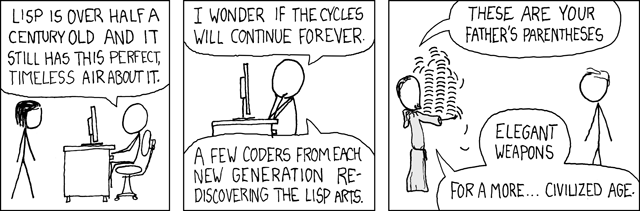
\includegraphics[width=\linewidth]{lisp_cycles.png}
      \caption{from \href{http://xkcd.com/297/}{XKCD}}
      \end{figure}
      \begin{itemize}
      \item Well, Common Lisp does have a lot\ldots
      \item \ldots but Clojure reduces them, uses vector square brackets, too
      \item Overall, Clojure has same or less parens+brackets+braces
        than many other languages (less
        code!)\\
{\ttfamily\color{black}
%
objA.method(b, c, d);}\\
$\Downarrow$\\
{\ttfamily\color{black}
\textcolor[rgb]{0.54901963,0.54901963,0.54901963}{(}function a b c d\textcolor[rgb]{0.54901963,0.54901963,0.54901963}{)}}
      \item Using Paredit mode (or equivalent) makes editing easy and
        having imbalanced parens difficult\\
        \begin{figure}
          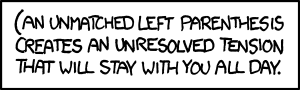
\includegraphics[width=0.8\linewidth]{left-paren.png}
          \caption{from \href{http://xkcd.com/859/}{XKCD}}
        \end{figure}
      \end{itemize}
    \item Commas are whitespace
      \begin{itemize}
      \item Useful for macros
      \end{itemize}
    \end{itemize}
  \item Java
    \begin{itemize}
    \item There is a lot of code
      \begin{figure}
        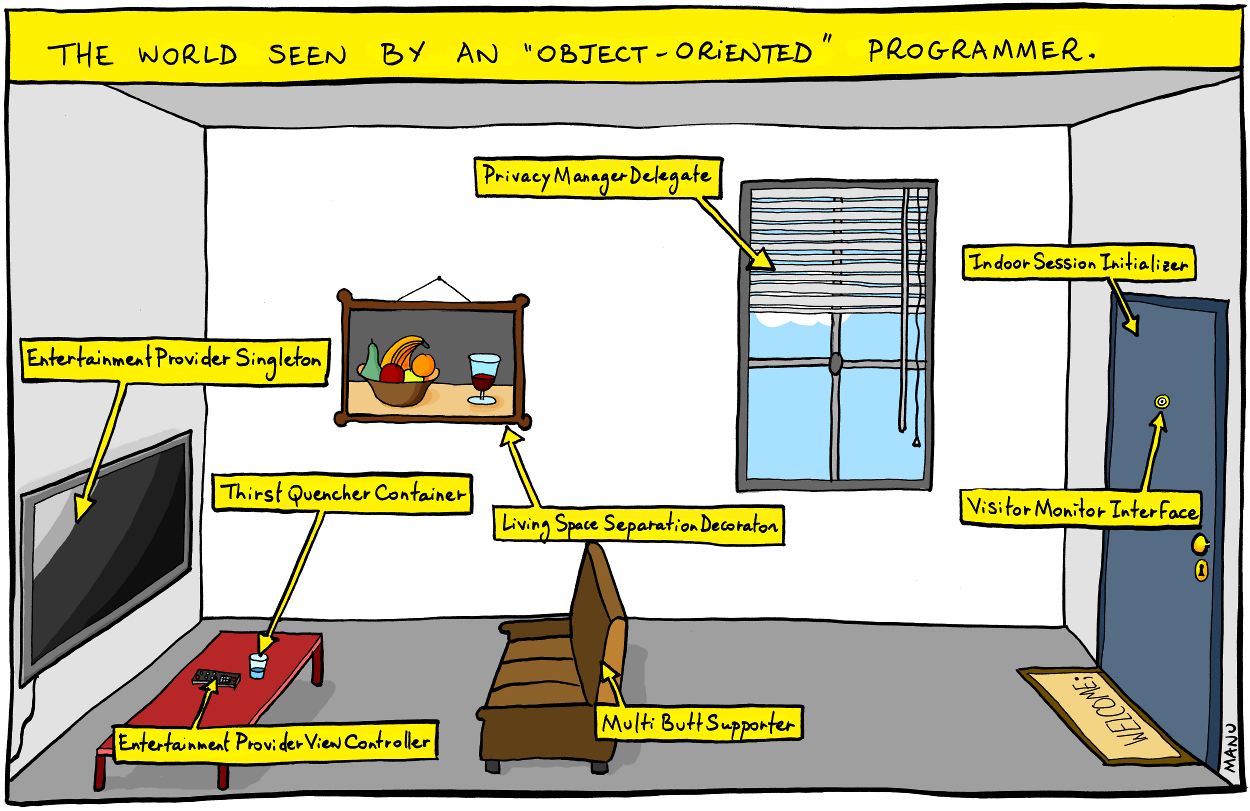
\includegraphics[width=\linewidth]{object_oriented_programmer_world.png}
        \caption{from \href{http://www.bonkersworld.net/object-world/}{Bonkers World}}
      \end{figure}
    \end{itemize}
  \item Ruby\\
    \begin{itemize}
    \item fn call parens can be omitted when the result is not
      ambiguous
    \item semicolon optional at end of the line 
    \end{itemize}
{\ttfamily\color{black}
%
\textcolor[rgb]{0.0,0.0,0.8039216}{{\textgreater} }\textbf{def
add\_two(x)}}

{\ttfamily\color{black}
\textcolor[rgb]{0.0,0.0,0.8039216}{{\textgreater} }\ \ \textbf{x + 2}}

{\ttfamily\color{black}
\textcolor[rgb]{0.0,0.0,0.8039216}{{\textgreater} }\textbf{end}}

{\ttfamily\color{black}
={\textgreater} nil}

{\ttfamily\color{black}
\textcolor[rgb]{0.0,0.0,0.8039216}{{\textgreater} }\textbf{add\_two 6}}

{\ttfamily\color{black}
={\textgreater} 8}
  \item Scala
    \begin{itemize}
    \item Type declarations go after a variable / function name, not
      in front
      \begin{itemize}
      \item Omissible when type can be inferred
      \end{itemize}
    \item fn call parens can be omitted when the result is not
      ambiguous
    \item Semicolon optional at end of line
    \end{itemize}
{\ttfamily\color{black}}
  \end{itemize}
\end{frame}

\begin{frame}[allowframebreaks]{Data Structures}
  \begin{itemize}
  \item 4 basic data structures with literal support in Clojure: lists, vectors,
    maps, sets
    \begin{itemize}
    \item List: {\ttfamily(1 1 2 3)}
    \item Vector: {\ttfamily[1 1 2 3]}
    \item Set: {\ttfamily \#\{1 2 3\}}
    \item Map: {\ttfamily \{\textquotedbl eins\textquotedbl\  1,
      \textquotedbl zwei\textquotedbl\ 2, \textquotedbl
      drei\textquotedbl\ 3 \}}
    \end{itemize}
  \item A lot of data can be represented through composites of these
  \item Functions are executed through lists (fn is in first position)

    \framebreak
  \item Clojure\\
\begin{small}
{\ttfamily\color{black}
%
\textcolor[rgb]{0.54901963,0.54901963,0.54901963}{(}\textcolor[rgb]{0.49803922,0.0,0.49803922}{def}
\textcolor{blue}{l}
\textcolor[rgb]{0.54901963,0.54901963,0.54901963}{(}\textcolor[rgb]{0.28235295,0.23921569,0.54509807}{list}
1 1 2 3\textcolor[rgb]{0.54901963,0.54901963,0.54901963}{))}}

{\ttfamily\color{black}
l}

{\ttfamily\color{black}
\textcolor[rgb]{0.54901963,0.54901963,0.54901963}{(}\textcolor[rgb]{0.49803922,0.0,0.49803922}{def}
\textcolor{blue}{v} [1 1 2
3]\textcolor[rgb]{0.54901963,0.54901963,0.54901963}{)}}

{\ttfamily\color{black}
v}

{\ttfamily\color{black}
\textcolor[rgb]{0.54901963,0.54901963,0.54901963}{(}\textcolor[rgb]{0.49803922,0.0,0.49803922}{def}
\textcolor{blue}{s} \#\{1 2
3\}\textcolor[rgb]{0.54901963,0.54901963,0.54901963}{)}}

{\ttfamily\color{black}
s}

{\ttfamily\color{black}
\textcolor[rgb]{0.54901963,0.54901963,0.54901963}{(}\textcolor[rgb]{0.49803922,0.0,0.49803922}{def}
\textcolor{blue}{m}
\{\textcolor[rgb]{0.54509807,0.13333334,0.32156864}{{\textquotedbl}eins{\textquotedbl}}
1,
\textcolor[rgb]{0.54509807,0.13333334,0.32156864}{{\textquotedbl}zwei{\textquotedbl}}
2,
\textcolor[rgb]{0.54509807,0.13333334,0.32156864}{{\textquotedbl}drei{\textquotedbl}}
3\}\textcolor[rgb]{0.54901963,0.54901963,0.54901963}{)}}

{\ttfamily\color{black}
m}
\end{small}
  \item Java\\
\begin{small}
{\ttfamily\color{black}
%
\textcolor[rgb]{0.69803923,0.13333334,0.13333334}{// omitting plain
arrays}}

{\ttfamily\color{black}
\textcolor[rgb]{0.49803922,0.0,0.49803922}{import}
\textcolor[rgb]{0.0,0.54509807,0.54509807}{java}.\textcolor[rgb]{0.0,0.54509807,0.54509807}{util}.\textcolor[rgb]{0.13333334,0.54509807,0.13333334}{List};}

{\ttfamily\color{black}
\textcolor[rgb]{0.49803922,0.0,0.49803922}{import}
\textcolor[rgb]{0.0,0.54509807,0.54509807}{java}.\textcolor[rgb]{0.0,0.54509807,0.54509807}{util}.\textcolor[rgb]{0.13333334,0.54509807,0.13333334}{ArrayList};}

{\ttfamily\color{black}
\textcolor[rgb]{0.13333334,0.54509807,0.13333334}{List}
\textcolor[rgb]{0.627451,0.32156864,0.1764706}{l} =
\textcolor[rgb]{0.49803922,0.0,0.49803922}{new}
\textcolor[rgb]{0.13333334,0.54509807,0.13333334}{ArrayList}();}

{\ttfamily\color{black}
l.add(1); \textcolor[rgb]{0.69803923,0.13333334,0.13333334}{// only with
auto-boxing starting in Java 1.5 aka 5}}

{\ttfamily\color{black}
l.add(1);}

{\ttfamily\color{black}
l.add(2);}

{\ttfamily\color{black}
l.add(3);}

{\ttfamily\color{black}
System.out.println(l);}

{\ttfamily\color{black}
\textcolor[rgb]{0.69803923,0.13333334,0.13333334}{// [1, 1, 2, 3]}}

{\ttfamily\color{black}
\textcolor[rgb]{0.13333334,0.54509807,0.13333334}{ArrayList}
\textcolor[rgb]{0.627451,0.32156864,0.1764706}{v} =
\textcolor[rgb]{0.49803922,0.0,0.49803922}{new}
\textcolor[rgb]{0.13333334,0.54509807,0.13333334}{ArrayList}();
\textcolor[rgb]{0.69803923,0.13333334,0.13333334}{// ArrayList replaced
Vector in Java 1.2}}


\bigskip

{\ttfamily\color{black}
%
\textcolor[rgb]{0.49803922,0.0,0.49803922}{import}
\textcolor[rgb]{0.0,0.54509807,0.54509807}{java}.\textcolor[rgb]{0.0,0.54509807,0.54509807}{util}.\textcolor[rgb]{0.13333334,0.54509807,0.13333334}{Set};}

{\ttfamily\color{black}
\textcolor[rgb]{0.49803922,0.0,0.49803922}{import}
\textcolor[rgb]{0.0,0.54509807,0.54509807}{java}.\textcolor[rgb]{0.0,0.54509807,0.54509807}{util}.\textcolor[rgb]{0.13333334,0.54509807,0.13333334}{HashSet};}

{\ttfamily\color{black}
\textcolor[rgb]{0.13333334,0.54509807,0.13333334}{Set}
\textcolor[rgb]{0.627451,0.32156864,0.1764706}{s} =
\textcolor[rgb]{0.49803922,0.0,0.49803922}{new}
\textcolor[rgb]{0.13333334,0.54509807,0.13333334}{HashSet}();}

{\ttfamily\color{black}
set.add(1);}

{\ttfamily\color{black}
set.add(2);}

{\ttfamily\color{black}
set.add(3);}

{\ttfamily\color{black}
System.out.println(s);}

{\ttfamily\color{black}
\textcolor[rgb]{0.69803923,0.13333334,0.13333334}{// [1, 2, 3]}}


\bigskip

{\ttfamily\color{black}
\textcolor[rgb]{0.49803922,0.0,0.49803922}{import}
\textcolor[rgb]{0.0,0.54509807,0.54509807}{java}.\textcolor[rgb]{0.0,0.54509807,0.54509807}{util}.\textcolor[rgb]{0.13333334,0.54509807,0.13333334}{Map};}

{\ttfamily\color{black}
\textcolor[rgb]{0.49803922,0.0,0.49803922}{import}
\textcolor[rgb]{0.0,0.54509807,0.54509807}{java}.\textcolor[rgb]{0.0,0.54509807,0.54509807}{util}.\textcolor[rgb]{0.13333334,0.54509807,0.13333334}{HashMap};}

{\ttfamily\color{black}
\textcolor[rgb]{0.13333334,0.54509807,0.13333334}{Map}
\textcolor[rgb]{0.627451,0.32156864,0.1764706}{m} =
\textcolor[rgb]{0.49803922,0.0,0.49803922}{new}
\textcolor[rgb]{0.13333334,0.54509807,0.13333334}{HashMap}();}

{\ttfamily\color{black}
m.put(\textcolor[rgb]{0.54509807,0.13333334,0.32156864}{{\textquotedbl}eins{\textquotedbl}},
1);}

{\ttfamily\color{black}
m.put(\textcolor[rgb]{0.54509807,0.13333334,0.32156864}{{\textquotedbl}zwei{\textquotedbl}},
2);}

{\ttfamily\color{black}
m.put(\textcolor[rgb]{0.54509807,0.13333334,0.32156864}{{\textquotedbl}drei{\textquotedbl}},
3);}

{\ttfamily\color{black}
System.out.println(m);}

{\ttfamily\color{black}
\textcolor[rgb]{0.69803923,0.13333334,0.13333334}{// \{zwei=2, drei=3,
eins=1\}}}
\end{small}
  \item Ruby\\
\begin{small}
{\ttfamily\color{black}
%
v = [1, 2, 3]}

{\ttfamily\color{black}
v}

{\ttfamily\color{black}
s = \textcolor[rgb]{0.13333334,0.54509807,0.13333334}{Set}.new([1, 2])}

{\ttfamily\color{black}
s}

{\ttfamily\color{black}
m =
\{\textcolor[rgb]{0.54509807,0.13333334,0.32156864}{{\textquotedbl}eins{\textquotedbl}}
={\textgreater} 1,
\textcolor[rgb]{0.54509807,0.13333334,0.32156864}{{\textquotedbl}zwei{\textquotedbl}}
={\textgreater} 2,
\textcolor[rgb]{0.54509807,0.13333334,0.32156864}{{\textquotedbl}drei{\textquotedbl}}
={\textgreater} 3\}}

{\ttfamily\color{black}
m}
\end{small}
  \item Scala\\
\begin{small}
{\ttfamily\color{black}
%
\textcolor[rgb]{0.49803922,0.0,0.49803922}{val}
\textcolor[rgb]{0.627451,0.32156864,0.1764706}{l} = List(1, 2, 3)}

{\ttfamily\color{black}
\textcolor[rgb]{0.49803922,0.0,0.49803922}{val}
\textcolor[rgb]{0.627451,0.32156864,0.1764706}{l2} = 1 :: 2 :: 3 ::
List()}

{\ttfamily\color{black}
l}

{\ttfamily\color{black}
\textcolor[rgb]{0.49803922,0.0,0.49803922}{val}
\textcolor[rgb]{0.627451,0.32156864,0.1764706}{v} = Vector(1, 2, 3)}

{\ttfamily\color{black}
v}

{\ttfamily\color{black}
\textcolor[rgb]{0.49803922,0.0,0.49803922}{val}
\textcolor[rgb]{0.627451,0.32156864,0.1764706}{s} = Set(1, 2, 3)}

{\ttfamily\color{black}
s}

{\ttfamily\color{black}
\textcolor[rgb]{0.49803922,0.0,0.49803922}{val}
\textcolor[rgb]{0.627451,0.32156864,0.1764706}{m} =
Map(\textcolor[rgb]{0.54509807,0.13333334,0.32156864}{{\textquotedbl}eins{\textquotedbl}}
-{\textgreater} 1,
\textcolor[rgb]{0.54509807,0.13333334,0.32156864}{{\textquotedbl}zwei{\textquotedbl}}
-{\textgreater} 2,
\textcolor[rgb]{0.54509807,0.13333334,0.32156864}{{\textquotedbl}drei{\textquotedbl}}
-{\textgreater} 3)}

{\ttfamily\color{black}
m}
\end{small}
  \end{itemize}
\end{frame}

\begin{frame}[allowframebreaks]{Immutability}
  \begin{itemize}
  \item Values don't change after declared
  \item Clojure
    \begin{itemize}
    \item Data structures (and any other value) are immutable
    \item Try:\\
\begin{small}
{\ttfamily\color{black}
%
\textcolor[rgb]{0.54901963,0.54901963,0.54901963}{(}\textcolor[rgb]{0.49803922,0.0,0.49803922}{def}
\textcolor{blue}{v1} [5
6]\textcolor[rgb]{0.54901963,0.54901963,0.54901963}{)}}

{\ttfamily\color{black}
\textcolor[rgb]{0.54901963,0.54901963,0.54901963}{(}\textcolor[rgb]{0.49803922,0.0,0.49803922}{def}
\textcolor{blue}{v2} [7
8]\textcolor[rgb]{0.54901963,0.54901963,0.54901963}{)}}

{\ttfamily\color{black}
\textcolor[rgb]{0.54901963,0.54901963,0.54901963}{(}\textcolor[rgb]{0.28235295,0.23921569,0.54509807}{concat}
v1 v2\textcolor[rgb]{0.54901963,0.54901963,0.54901963}{)}}

{\ttfamily\color{black}
v1}

{\ttfamily\color{black}
v2}

{\ttfamily\color{black}
\textcolor[rgb]{0.54901963,0.54901963,0.54901963}{(}\textcolor[rgb]{0.49803922,0.0,0.49803922}{def}
\textcolor{blue}{m} \{9
\textcolor[rgb]{0.54509807,0.13333334,0.32156864}{{\textquotedbl}nine{\textquotedbl}},
8
\textcolor[rgb]{0.54509807,0.13333334,0.32156864}{{\textquotedbl}eight{\textquotedbl}}\}\textcolor[rgb]{0.54901963,0.54901963,0.54901963}{)}}

{\ttfamily\color{black}
\textcolor[rgb]{0.54901963,0.54901963,0.54901963}{(}\textcolor[rgb]{0.28235295,0.23921569,0.54509807}{assoc}
m 7
\textcolor[rgb]{0.54509807,0.13333334,0.32156864}{{\textquotedbl}seven{\textquotedbl}}\textcolor[rgb]{0.54901963,0.54901963,0.54901963}{)}}

{\ttfamily\color{black}
m}
\end{small}
    \end{itemize}
  \item Java
    \begin{itemize}
    \item People with experience say no such thing as ``somewhat
      immutable'' code
    \item No immutable data structures originally, except for Strings,
      actually\\
\begin{small}
{\ttfamily\color{black}
%
\textcolor[rgb]{0.13333334,0.54509807,0.13333334}{String}
\textcolor[rgb]{0.627451,0.32156864,0.1764706}{str1} =
\textcolor[rgb]{0.54509807,0.13333334,0.32156864}{{\textquotedbl}hobnob
with Bob Loblaw{\textquotedbl}};}

{\ttfamily\color{black}
\textcolor[rgb]{0.13333334,0.54509807,0.13333334}{String}
\textcolor[rgb]{0.627451,0.32156864,0.1764706}{str2} =
\textcolor[rgb]{0.54509807,0.13333334,0.32156864}{{\textquotedbl} on
his Law Blog{\textquotedbl}};}

{\ttfamily\color{black}
str1.concat(str2);}

{\ttfamily\color{black}
System.out.println(\textcolor[rgb]{0.54509807,0.13333334,0.32156864}{{\textquotedbl}str1
= [{\textquotedbl}} + str1 +
\textcolor[rgb]{0.54509807,0.13333334,0.32156864}{{\textquotedbl}]{\textquotedbl}});}

{\ttfamily\color{black}
System.out.println(\textcolor[rgb]{0.54509807,0.13333334,0.32156864}{{\textquotedbl}str2
= [{\textquotedbl}} + str2 +
\textcolor[rgb]{0.54509807,0.13333334,0.32156864}{{\textquotedbl}]{\textquotedbl}});}

{\ttfamily\color{black}
\textcolor[rgb]{0.69803923,0.13333334,0.13333334}{// str1 = [hobnob with
Bob Loblaw]}}

{\ttfamily\color{black}
\textcolor[rgb]{0.69803923,0.13333334,0.13333334}{// str2 = [ on his Law
Blog]}}


\bigskip

{\ttfamily\color{black}
\textcolor[rgb]{0.13333334,0.54509807,0.13333334}{String}
\textcolor[rgb]{0.627451,0.32156864,0.1764706}{str3} =
str1.concat(str2);}

{\ttfamily\color{black}
System.out.println(\textcolor[rgb]{0.54509807,0.13333334,0.32156864}{{\textquotedbl}str1
= [{\textquotedbl}} + str1 +
\textcolor[rgb]{0.54509807,0.13333334,0.32156864}{{\textquotedbl}]{\textquotedbl}});}

{\ttfamily\color{black}
System.out.println(\textcolor[rgb]{0.54509807,0.13333334,0.32156864}{{\textquotedbl}str2
= [{\textquotedbl}} + str2 +
\textcolor[rgb]{0.54509807,0.13333334,0.32156864}{{\textquotedbl}]{\textquotedbl}});}

{\ttfamily\color{black}
System.out.println(\textcolor[rgb]{0.54509807,0.13333334,0.32156864}{{\textquotedbl}str3
= [{\textquotedbl}} + str3 +
\textcolor[rgb]{0.54509807,0.13333334,0.32156864}{{\textquotedbl}]{\textquotedbl}});}

{\ttfamily\color{black}
\textcolor[rgb]{0.69803923,0.13333334,0.13333334}{// str1 = [hobnob with
Bob Loblaw]}}

{\ttfamily\color{black}
\textcolor[rgb]{0.69803923,0.13333334,0.13333334}{// str2 = [ on his Law
Blog]}}

{\ttfamily\color{black}
\textcolor[rgb]{0.69803923,0.13333334,0.13333334}{// str3 = [hobnob with
Bob Loblaw on his Law Blog]}}
\end{small}
    \end{itemize}

    \framebreak
  \item Ruby
    \begin{itemize}
    \item Like Java, does not have immutable types
    \end{itemize}
  \item Scala\\
\begin{small}
{\ttfamily\color{black}
%
\textcolor[rgb]{0.0,0.0,0.8039216}{scala{\textgreater} }\textbf{val v1 =
Vector(5, 6)}}

{\ttfamily\color[rgb]{0.54509807,0.13333334,0.32156864}
v1: scala.collection.immutable.Vector[Int] = Vector(5, 6)}


\bigskip

{\ttfamily\color{black}
\textcolor[rgb]{0.0,0.0,0.8039216}{scala{\textgreater} }\textbf{val v2 =
Vector(7, 8)}}

{\ttfamily\color[rgb]{0.54509807,0.13333334,0.32156864}
v2: scala.collection.immutable.Vector[Int] = Vector(7, 8)}


\bigskip

{\ttfamily\color{black}
\textcolor[rgb]{0.0,0.0,0.8039216}{scala{\textgreater} }\textbf{v1 ++
v2}}

{\ttfamily\color[rgb]{0.54509807,0.13333334,0.32156864}
res1: scala.collection.immutable.Vector[Int] = Vector(5, 6, 7, 8)}


\bigskip

{\ttfamily\color{black}
\textcolor[rgb]{0.0,0.0,0.8039216}{scala{\textgreater} }\textbf{v1}}

{\ttfamily\color[rgb]{0.54509807,0.13333334,0.32156864}
res2: scala.collection.immutable.Vector[Int] = Vector(5, 6)}


\bigskip

{\ttfamily\color{black}
\textcolor[rgb]{0.0,0.0,0.8039216}{scala{\textgreater} }\textbf{v2}}

{\ttfamily\color[rgb]{0.54509807,0.13333334,0.32156864}
res3: scala.collection.immutable.Vector[Int] = Vector(7, 8)}


\bigskip

{\ttfamily\color{black}
\textcolor[rgb]{0.0,0.0,0.8039216}{scala{\textgreater} }\textbf{val m =
Map( 9 -{\textgreater} {\textquotedbl}nine{\textquotedbl}, 8
-{\textgreater} {\textquotedbl}eight{\textquotedbl})}}

{\ttfamily\color{black}
m: scala.collection.immutable.Map[Int,java.lang.String] = Map(9
\textcolor[rgb]{0.69803923,0.13333334,0.13333334}{{}-{\textgreater}}
nine, 8
\textcolor[rgb]{0.69803923,0.13333334,0.13333334}{{}-{\textgreater}}
eight)}


\bigskip

{\ttfamily\color{black}
\textcolor[rgb]{0.0,0.0,0.8039216}{scala{\textgreater} }\textbf{m + (7
-{\textgreater} {\textquotedbl}seven{\textquotedbl})}}

{\ttfamily\color{black}
res4: scala.collection.immutable.Map[Int,java.lang.String] = Map(9
\textcolor[rgb]{0.69803923,0.13333334,0.13333334}{{}-{\textgreater}}
nine, 8
\textcolor[rgb]{0.69803923,0.13333334,0.13333334}{{}-{\textgreater}}
eight, 7
\textcolor[rgb]{0.69803923,0.13333334,0.13333334}{{}-{\textgreater}}
seven)}


\bigskip

{\ttfamily\color{black}
\textcolor[rgb]{0.0,0.0,0.8039216}{scala{\textgreater} }\textbf{m}}

{\ttfamily\color{black}
res5: scala.collection.immutable.Map[Int,java.lang.String] = Map(9
\textcolor[rgb]{0.69803923,0.13333334,0.13333334}{{}-{\textgreater}}
nine, 8
\textcolor[rgb]{0.69803923,0.13333334,0.13333334}{{}-{\textgreater}}
eight)}
\end{small}


    \framebreak
  \item Referential transparency
    \begin{itemize}
    \item Don't rebind symbols/names (bind fn results to new symbols)
    \item Any code that references a symbol (ex: \texttt{v1}) always
      sees same value
      \begin{itemize}
      \item ``Either it works (all the time) or it doesn't work at
        all'' happens more often
      \end{itemize}
    \end{itemize}
  \item Structural sharing through persistent data structures
    \begin{itemize}
    \item Any code creating a new value using \texttt{v1} reuses
      memory
      \begin{itemize}
      \item EX: copying, appending, subsets, etc.
      \end{itemize}
    \end{itemize} 

    \framebreak
  \item Value semantics
    \begin{itemize}
    \item Clojure\\
{\ttfamily\color{black}
%
\textcolor[rgb]{0.54901963,0.54901963,0.54901963}{(}\textcolor[rgb]{0.49803922,0.0,0.49803922}{def}
\textcolor{blue}{v3}
v1\textcolor[rgb]{0.54901963,0.54901963,0.54901963}{)}}

{\ttfamily\color{black}
v1}

{\ttfamily\color{black}
v3}

{\ttfamily\color{black}
\textcolor[rgb]{0.54901963,0.54901963,0.54901963}{(}\textcolor[rgb]{0.28235295,0.23921569,0.54509807}{=}
v1 v3\textcolor[rgb]{0.54901963,0.54901963,0.54901963}{)}}

{\ttfamily\color{black}
\textcolor[rgb]{0.54901963,0.54901963,0.54901963}{(}\textcolor[rgb]{0.28235295,0.23921569,0.54509807}{=}
v3 [5 6]\textcolor[rgb]{0.54901963,0.54901963,0.54901963}{)}}

{\ttfamily\color{black}
\textcolor[rgb]{0.54901963,0.54901963,0.54901963}{(}\textcolor[rgb]{0.49803922,0.0,0.49803922}{def}
\textcolor{blue}{v4} [1 [2
[3]]]\textcolor[rgb]{0.54901963,0.54901963,0.54901963}{)}}

{\ttfamily\color{black}
\textcolor[rgb]{0.54901963,0.54901963,0.54901963}{(}\textcolor[rgb]{0.49803922,0.0,0.49803922}{def}
\textcolor{blue}{v5} [2
[3]]\textcolor[rgb]{0.54901963,0.54901963,0.54901963}{)}}

{\ttfamily\color{black}
\textcolor[rgb]{0.54901963,0.54901963,0.54901963}{(}\textcolor[rgb]{0.28235295,0.23921569,0.54509807}{second}
v4\textcolor[rgb]{0.54901963,0.54901963,0.54901963}{)}}

{\ttfamily\color{black}
\textcolor[rgb]{0.54901963,0.54901963,0.54901963}{(}\textcolor[rgb]{0.28235295,0.23921569,0.54509807}{=}
v5
\textcolor[rgb]{0.54901963,0.54901963,0.54901963}{(}\textcolor[rgb]{0.28235295,0.23921569,0.54509807}{second}
v4\textcolor[rgb]{0.54901963,0.54901963,0.54901963}{))}}

    \item Scala\\
{\ttfamily\color{black}
%
\textcolor[rgb]{0.49803922,0.0,0.49803922}{val}
\textcolor[rgb]{0.627451,0.32156864,0.1764706}{v3} = v1}

{\ttfamily\color{black}
v1}

{\ttfamily\color{black}
v3}

{\ttfamily\color{black}
v1 == v3}

{\ttfamily\color{black}
v3 == Vector(5,6)}

{\ttfamily\color{black}
\textcolor[rgb]{0.49803922,0.0,0.49803922}{val}
\textcolor[rgb]{0.627451,0.32156864,0.1764706}{v4} = Vector(1,
Vector(2, Vector(3)))}

{\ttfamily\color{black}
\textcolor[rgb]{0.49803922,0.0,0.49803922}{val}
\textcolor[rgb]{0.627451,0.32156864,0.1764706}{v5} = \ Vector(2,
Vector(3))}

{\ttfamily\color{black}
v5 == v4(1)}

    \end{itemize}
  \item Immutable values can be safely used in sets and in map keys
    \begin{itemize}
    \item Whereas Java allows mutable objects in sets or map keys (unadvisable)
    \item Python disallows mutable objectslists in sets or map keys
    \end{itemize}
  \item In general, Clojure uniquely teases out
    \begin{itemize}
    \item State as value + time, and\ldots
    \item Identity transcends time
    \end{itemize}
  \end{itemize}
\end{frame}

\subsection{Tabular comparisons}

\begin{frame}{Java, Ruby, Scala, \& Clojure}
  \begin{tabular}{l || c | c | c | c}
    aspect & Java & Ruby & Scala & Clojure\\
    \hline
    \hline
    strong typing & Y & Y & Y & Y\\
    \hline
    dynamic typing & N & Y & N & Y\\
    \hline
    interpreter/REPL & N & Y & Y & Y\\
    \hline
    functional style & N & Y & Y & Y\\
    \hline
    ``fun web prog.'' & N & Y & Y & Y\\
    \hline
    good for CLI script & N & Y & N & N\\
    \hline
    efficient with memory & Y & N & Y & Y\\
    \hline
    true multi-threaded & Y & N & Y & Y\\
  \end{tabular}
\end{frame}

\begin{frame}[allowframebreaks]{Clojure $\leftrightarrow$ Scala}
% Getting word wrap in a table using tabularx package
% http://stackoverflow.com/questions/790932/how-to-wrap-text-in-latex-tables
  \begin{tabularx}{\linewidth}{l || c | c | X}
    aspect & Clojure & Scala & why? (Clojure)\\
    \hline
    \hline
    STM & yes & yes & does for concurrency what GC did for memory\\
    \hline
    OOP & not really & yes & ``It is better to have 100 functions
    operate on one data structure than 10 functions on 10 data
    structures.''\\
    \hline
    design patterns & no & ?? & equivalent outcomes done in other
    ways\\
    \hline
    FP & yes & sort of & fns compose and can be used as arguments to
    other fns\\
  \end{tabularx}

  \framebreak
  \begin{tabularx}{\linewidth}{X || c | c | X}
    aspect & Clojure & Scala & why? (Clojure)\\
    \hline
    \hline
    concurrency & yes & yes* (?) & Clojure designed for this from the
    beginning\\
    \hline
    persistent data structures & yes & yes & only reasonable way to
    support immutable data structures\\
    \hline
    sequence abstraction & yes & yes & fns on seqs : objects :: UNIX :
    DOS\\
    \hline
    syntax regularity & yes & sort of & nice for macros, readability
    (\& pasting into REPL)\\
    \hline
  \end{tabularx}

  \framebreak
  \begin{tabularx}{\linewidth}{X || c | c | X}
    aspect & Clojure & Scala & why? (Clojure)\\
    \hline
    \hline
    language extensibility (macros) & yes & yes* & abstract repetitive
    code not possible via fns and patterns\\
    \hline
    backwards compatibility & yes & yes* & Clojure is relatively very
    good at working with old version code\\
  \end{tabularx}
\end{frame}

\subsection{Clojure Code Building Blocks}

\begin{frame}{Defining a Function}
  \begin{itemize}[<+->]
  \item Basic structure of a new fn\\
{\ttfamily\color{black}
%
\textcolor[rgb]{0.54901963,0.54901963,0.54901963}{(}\textcolor[rgb]{0.49803922,0.0,0.49803922}{defn}
\textcolor{blue}{fn-name}}

{\ttfamily\color{black}
\ \ \textcolor[rgb]{0.54509807,0.13333334,0.32156864}{{\textquotedbl}documentation
string{\textquotedbl}}}

{\ttfamily\color{black}
\ \ [arg1 arg2]}

{\ttfamily\color{black}
\ \ \textcolor[rgb]{0.69803923,0.13333334,0.13333334}{;; return value is
last form}}

{\ttfamily\color{black}
\ \ \textcolor[rgb]{0.54901963,0.54901963,0.54901963}{)}}
  \item Enter the following (in Light Table, if possible):\\
{\ttfamily\color{black}
%
\textcolor[rgb]{0.54901963,0.54901963,0.54901963}{(}\textcolor[rgb]{0.49803922,0.0,0.49803922}{defn}
\textcolor{blue}{square}}

{\ttfamily\color{black}
\ \ [x]}

{\ttfamily\color{black}
\ \ \textcolor[rgb]{0.54901963,0.54901963,0.54901963}{(}\textcolor[rgb]{0.28235295,0.23921569,0.54509807}{*}
x x\textcolor[rgb]{0.54901963,0.54901963,0.54901963}{))}}
  \item Now enter:\\
{\ttfamily\color{black}
%
\textcolor[rgb]{0.54901963,0.54901963,0.54901963}{(}square
2\textcolor[rgb]{0.54901963,0.54901963,0.54901963}{)}}

  \end{itemize}
\end{frame}

\begin{frame}[allowframebreaks]{Lexical scope - \texttt{let}}
  \begin{itemize}
  \item Can think of \texttt{let} form as giving ``local variables''
    \begin{itemize}
    \item Except they must all be declared at the beginning
    \end{itemize}
  \item The \texttt{let} bindings also used to break up a nested
    form into something more readable
  \item Example: Let's find the solutions of a quadratic equation
    \begin{itemize}
    \item For $ax^2 + bx + c = 0$, the solution is
\[x = \frac{-b \pm \sqrt{b^2 -4ac}}{2a}\]
    \item Test case:
\[a=1, b=-5, c=6\]
\[\Rightarrow x^2-5x+6 = 0\]
\[x=\lbrace2,3\rbrace\]
    \end{itemize}

    \framebreak
  \item First pass:\\
{\ttfamily\color{black}
%
\textcolor[rgb]{0.54901963,0.54901963,0.54901963}{(}\textcolor[rgb]{0.49803922,0.0,0.49803922}{defn}
\textcolor{blue}{quadsolve}}

{\ttfamily\color{black}
\ \ \textcolor[rgb]{0.54509807,0.13333334,0.32156864}{{\textquotedbl}solve
a quad eqn{\textquotedbl}}}

{\ttfamily\color{black}
\ \ [a b c]}

{\ttfamily\color{black}
\ \ [\textcolor[rgb]{0.54901963,0.54901963,0.54901963}{(}\textcolor[rgb]{0.28235295,0.23921569,0.54509807}{/}
\textcolor[rgb]{0.54901963,0.54901963,0.54901963}{(}\textcolor[rgb]{0.28235295,0.23921569,0.54509807}{+}
\textcolor[rgb]{0.54901963,0.54901963,0.54901963}{(}\textcolor[rgb]{0.28235295,0.23921569,0.54509807}{{}-}
b\textcolor[rgb]{0.54901963,0.54901963,0.54901963}{)}
\textcolor[rgb]{0.54901963,0.54901963,0.54901963}{(}\textcolor[rgb]{0.28235295,0.23921569,0.54509807}{{}-}
\textcolor[rgb]{0.54901963,0.54901963,0.54901963}{(}square
b\textcolor[rgb]{0.54901963,0.54901963,0.54901963}{)}
\textcolor[rgb]{0.54901963,0.54901963,0.54901963}{(}\textcolor[rgb]{0.28235295,0.23921569,0.54509807}{*}
4 a c\textcolor[rgb]{0.54901963,0.54901963,0.54901963}{)))}
\textcolor[rgb]{0.54901963,0.54901963,0.54901963}{(}\textcolor[rgb]{0.28235295,0.23921569,0.54509807}{*}
2 a\textcolor[rgb]{0.54901963,0.54901963,0.54901963}{))}
\textcolor[rgb]{0.54901963,0.54901963,0.54901963}{(}\textcolor[rgb]{0.28235295,0.23921569,0.54509807}{/}
\textcolor[rgb]{0.54901963,0.54901963,0.54901963}{(}\textcolor[rgb]{0.28235295,0.23921569,0.54509807}{{}-}
\textcolor[rgb]{0.54901963,0.54901963,0.54901963}{(}\textcolor[rgb]{0.28235295,0.23921569,0.54509807}{{}-}
b\textcolor[rgb]{0.54901963,0.54901963,0.54901963}{)}
\textcolor[rgb]{0.54901963,0.54901963,0.54901963}{(}\textcolor[rgb]{0.28235295,0.23921569,0.54509807}{{}-}
\textcolor[rgb]{0.54901963,0.54901963,0.54901963}{(}square
b\textcolor[rgb]{0.54901963,0.54901963,0.54901963}{)}
\textcolor[rgb]{0.54901963,0.54901963,0.54901963}{(}\textcolor[rgb]{0.28235295,0.23921569,0.54509807}{*}
4 a c\textcolor[rgb]{0.54901963,0.54901963,0.54901963}{)))}
\textcolor[rgb]{0.54901963,0.54901963,0.54901963}{(}\textcolor[rgb]{0.28235295,0.23921569,0.54509807}{*}
2
a\textcolor[rgb]{0.54901963,0.54901963,0.54901963}{))}]\textcolor[rgb]{0.54901963,0.54901963,0.54901963}{)}}


  \begin{itemize}
  \item Check:\\ 
{\ttfamily\color{black}
\textcolor[rgb]{0.54901963,0.54901963,0.54901963}{(}quadsolve 1 -5
6\textcolor[rgb]{0.54901963,0.54901963,0.54901963}{)}}
  \end{itemize}

    \framebreak
  \item Define:\\

{\ttfamily\color{black}
\textcolor[rgb]{0.54901963,0.54901963,0.54901963}{(}\textcolor[rgb]{0.49803922,0.0,0.49803922}{defn}
\textcolor{blue}{discriminant}}

{\ttfamily\color{black}
\ \ \textcolor[rgb]{0.54509807,0.13333334,0.32156864}{{\textquotedbl}for
a quadratic eqn{\textquotesingle}s coefficients, return the
discriminant{\textquotedbl}}}

{\ttfamily\color{black}
\ \ [a b c]}

{\ttfamily\color{black}
\ \ \textcolor[rgb]{0.54901963,0.54901963,0.54901963}{(}\textcolor[rgb]{0.28235295,0.23921569,0.54509807}{{}-}
\textcolor[rgb]{0.54901963,0.54901963,0.54901963}{(}square
b\textcolor[rgb]{0.54901963,0.54901963,0.54901963}{)}
\textcolor[rgb]{0.54901963,0.54901963,0.54901963}{(}\textcolor[rgb]{0.28235295,0.23921569,0.54509807}{*}
4 a c\textcolor[rgb]{0.54901963,0.54901963,0.54901963}{)))}}

    \begin{itemize}
    \item Check:\\
      {\ttfamily\color{black}
      \textcolor[rgb]{0.54901963,0.54901963,0.54901963}{(}discriminant 1 -5
      6\textcolor[rgb]{0.54901963,0.54901963,0.54901963}{)}} 
    \end{itemize}

  \item Rewrite:\\
{\ttfamily\color{black}
\textcolor[rgb]{0.54901963,0.54901963,0.54901963}{(}\textcolor[rgb]{0.49803922,0.0,0.49803922}{defn}
\textcolor{blue}{quadsolve}}

{\ttfamily\color{black}
\ \ [a b c]}

{\ttfamily\color{black}
\ \ \textcolor[rgb]{0.54901963,0.54901963,0.54901963}{(}\textcolor[rgb]{0.49803922,0.0,0.49803922}{let}
[disc \textcolor[rgb]{0.54901963,0.54901963,0.54901963}{(}discriminant
a b c\textcolor[rgb]{0.54901963,0.54901963,0.54901963}{)}}

{\ttfamily\color{black}
\ \ \ \ \ \ \ \ disc-sqrt
\textcolor[rgb]{0.54901963,0.54901963,0.54901963}{(}\textcolor[rgb]{0.28235295,0.23921569,0.54509807}{Math/sqrt}
disc\textcolor[rgb]{0.54901963,0.54901963,0.54901963}{)}]}

{\ttfamily\color{black}
\ \ \ \ [\textcolor[rgb]{0.54901963,0.54901963,0.54901963}{(}\textcolor[rgb]{0.28235295,0.23921569,0.54509807}{/}
\textcolor[rgb]{0.54901963,0.54901963,0.54901963}{(}\textcolor[rgb]{0.28235295,0.23921569,0.54509807}{+}
\textcolor[rgb]{0.54901963,0.54901963,0.54901963}{(}\textcolor[rgb]{0.28235295,0.23921569,0.54509807}{{}-}
b\textcolor[rgb]{0.54901963,0.54901963,0.54901963}{)}
disc-sqrt\textcolor[rgb]{0.54901963,0.54901963,0.54901963}{)}
\textcolor[rgb]{0.54901963,0.54901963,0.54901963}{(}\textcolor[rgb]{0.28235295,0.23921569,0.54509807}{*}
2 a\textcolor[rgb]{0.54901963,0.54901963,0.54901963}{))}
\textcolor[rgb]{0.54901963,0.54901963,0.54901963}{(}\textcolor[rgb]{0.28235295,0.23921569,0.54509807}{/}
\textcolor[rgb]{0.54901963,0.54901963,0.54901963}{(}\textcolor[rgb]{0.28235295,0.23921569,0.54509807}{{}-}
\textcolor[rgb]{0.54901963,0.54901963,0.54901963}{(}\textcolor[rgb]{0.28235295,0.23921569,0.54509807}{{}-}
b\textcolor[rgb]{0.54901963,0.54901963,0.54901963}{)}
disc-sqrt\textcolor[rgb]{0.54901963,0.54901963,0.54901963}{)}
\textcolor[rgb]{0.54901963,0.54901963,0.54901963}{(}\textcolor[rgb]{0.28235295,0.23921569,0.54509807}{*}
2
a\textcolor[rgb]{0.54901963,0.54901963,0.54901963}{))}]\textcolor[rgb]{0.54901963,0.54901963,0.54901963}{))}}


  \begin{itemize}
  \item \texttt{Math/sqrt} refers to the \texttt{sqrt} static method
    of Java's \texttt{java.lang.Math}
  \item Check:\\
{\ttfamily\color{black}
\textcolor[rgb]{0.54901963,0.54901963,0.54901963}{(}quadsolve 1 -5
6\textcolor[rgb]{0.54901963,0.54901963,0.54901963}{)}}
  \end{itemize}

  \end{itemize}
\end{frame}

\begin{frame}[allowframebreaks]{Control Flow - \texttt{if}, etc.}
  \begin{itemize}
  \item \texttt{if}
    \begin{itemize}
    \item Takes a 3 expressions: a test, the ``then'', and the
      ``else''
    \item Note: test passes for all values except \texttt{false} and
      \texttt{nil}
      \begin{itemize}
      \item This ``truthiness'' holds for everything built off of
        \texttt{if} - \texttt{when, and, or, if-not, when-not}, etc.
      \end{itemize}
    \item 
{\ttfamily\color{black}
%
\textcolor[rgb]{0.54901963,0.54901963,0.54901963}{(}\textcolor[rgb]{0.49803922,0.0,0.49803922}{if}
\textcolor[rgb]{0.54901963,0.54901963,0.54901963}{(}\textcolor[rgb]{0.28235295,0.23921569,0.54509807}{{\textless}}
disc 0\textcolor[rgb]{0.54901963,0.54901963,0.54901963}{)}}

{\ttfamily\color{black}
\ \ \textcolor[rgb]{0.54901963,0.54901963,0.54901963}{(}\textcolor[rgb]{0.28235295,0.23921569,0.54509807}{println}
\textcolor[rgb]{0.54509807,0.13333334,0.32156864}{{\textquotedbl}I
don{\textquotesingle}t like imaginary
numbers!{\textquotedbl}}\textcolor[rgb]{0.54901963,0.54901963,0.54901963}{)}}

{\ttfamily\color{black}
\ \ [\textcolor[rgb]{0.54901963,0.54901963,0.54901963}{(}\textcolor[rgb]{0.28235295,0.23921569,0.54509807}{/}
\textcolor[rgb]{0.54901963,0.54901963,0.54901963}{(}\textcolor[rgb]{0.28235295,0.23921569,0.54509807}{+}
\textcolor[rgb]{0.54901963,0.54901963,0.54901963}{(}\textcolor[rgb]{0.28235295,0.23921569,0.54509807}{{}-}
b\textcolor[rgb]{0.54901963,0.54901963,0.54901963}{)}
disc-sqrt\textcolor[rgb]{0.54901963,0.54901963,0.54901963}{)}
\textcolor[rgb]{0.54901963,0.54901963,0.54901963}{(}\textcolor[rgb]{0.28235295,0.23921569,0.54509807}{*}
2 a\textcolor[rgb]{0.54901963,0.54901963,0.54901963}{))}
\textcolor[rgb]{0.54901963,0.54901963,0.54901963}{(}\textcolor[rgb]{0.28235295,0.23921569,0.54509807}{/}
\textcolor[rgb]{0.54901963,0.54901963,0.54901963}{(}\textcolor[rgb]{0.28235295,0.23921569,0.54509807}{{}-}
\textcolor[rgb]{0.54901963,0.54901963,0.54901963}{(}\textcolor[rgb]{0.28235295,0.23921569,0.54509807}{{}-}
b\textcolor[rgb]{0.54901963,0.54901963,0.54901963}{)}
disc-sqrt\textcolor[rgb]{0.54901963,0.54901963,0.54901963}{)}
\textcolor[rgb]{0.54901963,0.54901963,0.54901963}{(}\textcolor[rgb]{0.28235295,0.23921569,0.54509807}{*}
2
a\textcolor[rgb]{0.54901963,0.54901963,0.54901963}{))}]\textcolor[rgb]{0.54901963,0.54901963,0.54901963}{)}}
    \end{itemize}
  \item \texttt{do}
    \begin{itemize}
    \item Creates a form that evaluates/executes multiple forms inside it
    \item Returns the value of the last form\\
{\ttfamily\color{black}
\textcolor[rgb]{0.54901963,0.54901963,0.54901963}{(}\textcolor[rgb]{0.49803922,0.0,0.49803922}{if}
\textcolor[rgb]{0.54901963,0.54901963,0.54901963}{(}\textcolor[rgb]{0.28235295,0.23921569,0.54509807}{{\textless}}
disc 0\textcolor[rgb]{0.54901963,0.54901963,0.54901963}{)}}

{\ttfamily\color{black}
\ \ \textcolor[rgb]{0.54901963,0.54901963,0.54901963}{(}\textcolor[rgb]{0.28235295,0.23921569,0.54509807}{println}
\textcolor[rgb]{0.54509807,0.13333334,0.32156864}{{\textquotedbl}I
don{\textquotesingle}t like imaginary
numbers{\textquotedbl}}\textcolor[rgb]{0.54901963,0.54901963,0.54901963}{)}}

{\ttfamily\color{black}
\ \ \textcolor[rgb]{0.54901963,0.54901963,0.54901963}{(}\textcolor[rgb]{0.49803922,0.0,0.49803922}{do}}

{\ttfamily\color{black}
\ \ \ \ \textcolor[rgb]{0.54901963,0.54901963,0.54901963}{(}\textcolor[rgb]{0.28235295,0.23921569,0.54509807}{println}
\textcolor[rgb]{0.54509807,0.13333334,0.32156864}{{\textquotedbl}I like
real
numbers!{\textquotedbl}}\textcolor[rgb]{0.54901963,0.54901963,0.54901963}{)}}

{\ttfamily\color{black}
\ \ \ \ [\textcolor[rgb]{0.54901963,0.54901963,0.54901963}{(}\textcolor[rgb]{0.28235295,0.23921569,0.54509807}{/}
\textcolor[rgb]{0.54901963,0.54901963,0.54901963}{(}\textcolor[rgb]{0.28235295,0.23921569,0.54509807}{+}
\textcolor[rgb]{0.54901963,0.54901963,0.54901963}{(}\textcolor[rgb]{0.28235295,0.23921569,0.54509807}{{}-}
b\textcolor[rgb]{0.54901963,0.54901963,0.54901963}{)}
disc-sqrt\textcolor[rgb]{0.54901963,0.54901963,0.54901963}{)}
\textcolor[rgb]{0.54901963,0.54901963,0.54901963}{(}\textcolor[rgb]{0.28235295,0.23921569,0.54509807}{*}
2 a\textcolor[rgb]{0.54901963,0.54901963,0.54901963}{))}
\textcolor[rgb]{0.54901963,0.54901963,0.54901963}{(}\textcolor[rgb]{0.28235295,0.23921569,0.54509807}{/}
\textcolor[rgb]{0.54901963,0.54901963,0.54901963}{(}\textcolor[rgb]{0.28235295,0.23921569,0.54509807}{{}-}
\textcolor[rgb]{0.54901963,0.54901963,0.54901963}{(}\textcolor[rgb]{0.28235295,0.23921569,0.54509807}{{}-}
b\textcolor[rgb]{0.54901963,0.54901963,0.54901963}{)}
disc-sqrt\textcolor[rgb]{0.54901963,0.54901963,0.54901963}{)}
\textcolor[rgb]{0.54901963,0.54901963,0.54901963}{(}\textcolor[rgb]{0.28235295,0.23921569,0.54509807}{*}
2
a\textcolor[rgb]{0.54901963,0.54901963,0.54901963}{))}]\textcolor[rgb]{0.54901963,0.54901963,0.54901963}{))}}

    \end{itemize}
  \item \texttt{when} is the same as \texttt{if}, but with
    \texttt{nil} as ``else'' and a
    \texttt{do} built in for ``then''
  \item Both \texttt{and} and \texttt{or} do short-circuit evaluation
  \end{itemize}
\end{frame}


\begin{frame}[allowframebreaks]{\texttt{map} \& \texttt{reduce}}
  \begin{itemize}
  \item Where's my for loop??
    \begin{itemize}
    \item Instead of dealing with index-based looping, you can apply
      higher-order functions
    \end{itemize}
  \item \texttt{map} applies a fn on every element of a sequence
  \item \texttt{reduce} uses a fn to accumulate an answer
    \begin{itemize}
    \item Apply fn on first 2 elements (or an initial value and first
      element)
    \item Continue applying fn on accumulated value and next element
    \end{itemize}


  \framebreak
\begin{small}
{\ttfamily\color{black}
%
\textcolor[rgb]{0.49803922,0.0,0.49803922}{user{\textgreater}
}\textbf{(def data [3 5 9 1 5 4 2])}}

{\ttfamily\color{black}
\#{\textquotesingle}user/data}

{\ttfamily\color{black}
\textcolor[rgb]{0.49803922,0.0,0.49803922}{user{\textgreater}
}\textbf{(map square data)}}

{\ttfamily\color{black}
(9 25 81 1 25 16 4)}

{\ttfamily\color{black}
\textcolor[rgb]{0.49803922,0.0,0.49803922}{user{\textgreater}
}\textbf{(reduce + data)}}

{\ttfamily\color{black}
29}

{\ttfamily\color{black}
\textcolor[rgb]{0.49803922,0.0,0.49803922}{user{\textgreater}
}\textbf{(defn sum-sq}}

{\ttfamily\color{black}
\ \ \ \ \ \ \ \ \ \textbf{[nums]}}

{\ttfamily\color{black}
\ \ \ \ \ \ \ \ \ \textbf{(reduce + (map
square nums)))}}

{\ttfamily\color{black}
\#{\textquotesingle}user/sum-sq}

{\ttfamily\color{black}
\textcolor[rgb]{0.49803922,0.0,0.49803922}{user{\textgreater}
}\textbf{(sum-sq data)}}

{\ttfamily\color{black}
161}
\end{small}

  \framebreak
  \item Since Clojure fns are first-class citizens
    \begin{itemize}
    \item You can have a vector of fns: \texttt{[+ -]}
    \item You can have an anonymous fn (doesn't have a name):\\
{\ttfamily\color{black}
%
\textcolor[rgb]{0.54901963,0.54901963,0.54901963}{(}\textcolor[rgb]{0.49803922,0.0,0.49803922}{fn}
[x]
\textcolor[rgb]{0.54901963,0.54901963,0.54901963}{(}\textcolor[rgb]{0.49803922,0.0,0.49803922}{if}
\textcolor[rgb]{0.54901963,0.54901963,0.54901963}{(}\textcolor[rgb]{0.28235295,0.23921569,0.54509807}{pos?}
x\textcolor[rgb]{0.54901963,0.54901963,0.54901963}{)} x
\textcolor[rgb]{0.54901963,0.54901963,0.54901963}{(}\textcolor[rgb]{0.28235295,0.23921569,0.54509807}{{}-}
x\textcolor[rgb]{0.54901963,0.54901963,0.54901963}{)))}}
    \end{itemize}
  \item Our next rewrite of \texttt{quadsolve}:\\
{\ttfamily\color{black}
%
\textcolor[rgb]{0.54901963,0.54901963,0.54901963}{(}\textcolor[rgb]{0.49803922,0.0,0.49803922}{defn}
\textcolor{blue}{quadsolve}}

{\ttfamily\color{black}
\ \ [a b c]}

{\ttfamily\color{black}
\ \ \textcolor[rgb]{0.54901963,0.54901963,0.54901963}{(}\textcolor[rgb]{0.49803922,0.0,0.49803922}{let}
[disc \textcolor[rgb]{0.54901963,0.54901963,0.54901963}{(}discriminant
a b c\textcolor[rgb]{0.54901963,0.54901963,0.54901963}{)}}

{\ttfamily\color{black}
\ \ \ \ \ \ \ \ disc-sqrt
\textcolor[rgb]{0.54901963,0.54901963,0.54901963}{(}\textcolor[rgb]{0.28235295,0.23921569,0.54509807}{Math/sqrt}
disc\textcolor[rgb]{0.54901963,0.54901963,0.54901963}{)}}

{\ttfamily\color{black}
\ \ \ \ \ \ \ \ soln-fn
\textcolor[rgb]{0.54901963,0.54901963,0.54901963}{(}\textcolor[rgb]{0.49803922,0.0,0.49803922}{fn}
[op]
\textcolor[rgb]{0.54901963,0.54901963,0.54901963}{(}\textcolor[rgb]{0.28235295,0.23921569,0.54509807}{/}
\textcolor[rgb]{0.54901963,0.54901963,0.54901963}{(}op
\textcolor[rgb]{0.54901963,0.54901963,0.54901963}{(}\textcolor[rgb]{0.28235295,0.23921569,0.54509807}{{}-}
b\textcolor[rgb]{0.54901963,0.54901963,0.54901963}{)}
disc-sqrt\textcolor[rgb]{0.54901963,0.54901963,0.54901963}{)}
\textcolor[rgb]{0.54901963,0.54901963,0.54901963}{(}\textcolor[rgb]{0.28235295,0.23921569,0.54509807}{*}
2 a\textcolor[rgb]{0.54901963,0.54901963,0.54901963}{)))}}

{\ttfamily\color{black}
\ \ \ \ \ \ \ \ ops [+ -]]}

{\ttfamily\color{black}
\ \ \ \ \textcolor[rgb]{0.54901963,0.54901963,0.54901963}{(}\textcolor[rgb]{0.28235295,0.23921569,0.54509807}{map}
soln-fn ops\textcolor[rgb]{0.54901963,0.54901963,0.54901963}{)))}}
  \end{itemize}
\end{frame}

\begin{frame}{Closures}
  \begin{itemize}
  \item \texttt{soln-fn} is a closure -- the values of
    \texttt{a}, \texttt{b}, and \texttt{disc-sqrt} are pulled from surrounding scope
  \item Even if \texttt{soln-fn} is passed elsewhere, the values of
    \texttt{a}, \texttt{b}, and \texttt{disc-sqrt} in \texttt{soln-fn} don't change after fn creation \&
    binding 
    \begin{itemize}
    \item fns $\Rightarrow$ values $\Rightarrow$ immutable
    \end{itemize}
  \item Ex: you have to decrypt a lot of strings encrypted with the
    same public key
    \begin{itemize}
    \item Instead of repeated \texttt{(decrypt priv-key s \ldots)}
      calls\\
\begin{small}
{\ttfamily\color{black}
%
\textcolor[rgb]{0.54901963,0.54901963,0.54901963}{(}\textcolor[rgb]{0.49803922,0.0,0.49803922}{defn}
\textcolor{blue}{decrypt-with-priv}}

{\ttfamily\color{black}
\ \ [priv-key]}

{\ttfamily\color{black}
\ \ \textcolor[rgb]{0.54901963,0.54901963,0.54901963}{(}\textcolor[rgb]{0.49803922,0.0,0.49803922}{fn}
[s]}

{\ttfamily\color{black}
\ \ \ \ \textcolor[rgb]{0.54901963,0.54901963,0.54901963}{(}decrypt
priv-key s\textcolor[rgb]{0.54901963,0.54901963,0.54901963}{)))}}


\bigskip

{\ttfamily\color{black}
\textcolor[rgb]{0.54901963,0.54901963,0.54901963}{(}\textcolor[rgb]{0.49803922,0.0,0.49803922}{let}
[my-decrypt
\textcolor[rgb]{0.54901963,0.54901963,0.54901963}{(}decrypt-with-priv
priv-key\textcolor[rgb]{0.54901963,0.54901963,0.54901963}{)}]}

{\ttfamily\color{black}
\ \ \textcolor[rgb]{0.54901963,0.54901963,0.54901963}{(}my-decrypt
s1\textcolor[rgb]{0.54901963,0.54901963,0.54901963}{)}}

{\ttfamily\color{black}
\ \ \textcolor[rgb]{0.54901963,0.54901963,0.54901963}{(}my-decrypt
s2\textcolor[rgb]{0.54901963,0.54901963,0.54901963}{)}}

{\ttfamily\color{black}
\ \ \ldots\textcolor[rgb]{0.54901963,0.54901963,0.54901963}{)}}
\end{small}
    \item In many cases, as above, \texttt{partial} does the same
    \end{itemize}
  \end{itemize}
\end{frame}

\begin{frame}{Java Interop}
  \begin{itemize}
  \item Java classes in JVM and classpath accessible
    \begin{itemize}
    \item Use full name unless imported, ex: {\ttfamily\color{black}
%
\textcolor[rgb]{0.54901963,0.54901963,0.54901963}{(}\textcolor[rgb]{0.49803922,0.0,0.49803922}{import}
{\textquotesingle}\textcolor[rgb]{0.28235295,0.23921569,0.54509807}{java.net.URL}\textcolor[rgb]{0.54901963,0.54901963,0.54901963}{)}}
    \item All of \texttt{java.lang.*} always imported, just like Java
    \end{itemize}
  \item New objects through \texttt{new}: {\ttfamily\color{black}
%
\textcolor[rgb]{0.54901963,0.54901963,0.54901963}{(}new
\textcolor[rgb]{0.28235295,0.23921569,0.54509807}{URL}
\textcolor[rgb]{0.54509807,0.13333334,0.32156864}{{\textquotedbl}http://clojure.org{\textquotedbl}}\textcolor[rgb]{0.54901963,0.54901963,0.54901963}{)}}
    \begin{itemize}
    \item Syntax shorcut: {\ttfamily\color{black}
\textcolor[rgb]{0.54901963,0.54901963,0.54901963}{(}\textcolor[rgb]{0.28235295,0.23921569,0.54509807}{URL.}
\textcolor[rgb]{0.54509807,0.13333334,0.32156864}{{\textquotedbl}http://clojure.org{\textquotedbl}}\textcolor[rgb]{0.54901963,0.54901963,0.54901963}{)}}
    \end{itemize}
  \item Static methods called through \texttt{Class/method} (ex: {\ttfamily\color[rgb]{0.28235295,0.23921569,0.54509807}
Math/sqrt})
  \item Idiomatic member method call ex: {\ttfamily\color{black}
\textcolor[rgb]{0.54901963,0.54901963,0.54901963}{(}\textcolor[rgb]{0.28235295,0.23921569,0.54509807}{.toLowerCase}
\textcolor[rgb]{0.54509807,0.13333334,0.32156864}{{\textquotedbl}sUpEr
UgLy
CaSiNg{\textquotedbl}}\textcolor[rgb]{0.54901963,0.54901963,0.54901963}{)}}
  \item More (\& interesting) Java interop available (ex:
    \texttt{proxy}, \texttt{memfn}, etc.)
  \item Clojure way for Java patterns very neat (multimethods, protocols, records, types)
  \end{itemize}
\end{frame}






\begin{frame}[allowframebreaks]{Sequence/List Processing Functions}
  \begin{itemize}
  \item Many useful fns exist to transform sequences, work on specific
    collection types, or convert from one to another
  \item Examples:\\
{\ttfamily\color{black}
\textcolor[rgb]{0.49803922,0.0,0.49803922}{user{\textgreater}
}\textbf{(filter even? data)}}

{\ttfamily\color{black}
(4 2)}

{\ttfamily\color{black}
\textcolor[rgb]{0.49803922,0.0,0.49803922}{user{\textgreater}
}\textbf{(remove even? data)}}

{\ttfamily\color{black}
(3 5 9 1 5)}

{\ttfamily\color{black}
%
\textcolor[rgb]{0.49803922,0.0,0.49803922}{user{\textgreater}
}\textbf{(take 3 data)}}

{\ttfamily\color{black}
(3 5 9)}

{\ttfamily\color{black}
\textcolor[rgb]{0.49803922,0.0,0.49803922}{user{\textgreater}
}\textbf{(drop 3 data)}}

{\ttfamily\color{black}
(1 5 4 2)}

{\ttfamily\color{black}
\textcolor[rgb]{0.49803922,0.0,0.49803922}{user{\textgreater}
}\textbf{(first data)}}

{\ttfamily\color{black}
3}

{\ttfamily\color{black}
\textcolor[rgb]{0.49803922,0.0,0.49803922}{user{\textgreater}
}\textbf{(rest data)}}

{\ttfamily\color{black}
(5 9 1 5 4 2)}

{\ttfamily\color{black}
\textcolor[rgb]{0.49803922,0.0,0.49803922}{user{\textgreater}
}\textbf{(last data)}}

{\ttfamily\color{black}
2}

{\ttfamily\color{black}
\textcolor[rgb]{0.49803922,0.0,0.49803922}{user{\textgreater}
}\textbf{(butlast data)}}

{\ttfamily\color{black}
(3 5 9 1 5 4)}

{\ttfamily\color{black}
\textcolor[rgb]{0.49803922,0.0,0.49803922}{user{\textgreater}
}\textbf{(take-while (fn [x] ({\textless} 1 x)) data)}}

{\ttfamily\color{black}
(3 5 9)}

{\ttfamily\color{black}
\textcolor[rgb]{0.49803922,0.0,0.49803922}{user{\textgreater}
}\textbf{(drop-while (fn [x] ({\textless} 1 x)) data)}}

{\ttfamily\color{black}
(1 5 4 2)}

{\ttfamily\color{black}
\textcolor[rgb]{0.49803922,0.0,0.49803922}{user{\textgreater}
}\textbf{(take-nth 2 data)}}

{\ttfamily\color{black}
(3 9 5 2)}


  \framebreak


{\ttfamily\color{black}
%
\textcolor[rgb]{0.49803922,0.0,0.49803922}{user{\textgreater}
}\textbf{(def nums [1 1 1 2 1 1 2 1 1 1 1 1 2 2 1 3 1 2 2 1 1])}}

{\ttfamily\color{black}
\#{\textquotesingle}user/nums}

{\ttfamily\color{black}
%
\textcolor[rgb]{0.49803922,0.0,0.49803922}{user{\textgreater}
}\textbf{(frequencies nums)}}

{\ttfamily\color{black}
\{1 13, 2 6, 3 1\}}

{\ttfamily\color{black}
\textcolor[rgb]{0.49803922,0.0,0.49803922}{user{\textgreater}
}\textbf{(group-by odd? nums)}}

{\ttfamily\color{black}
\{true [1 1 1 1 1 1 1 1 1 1 3 1 1 1], false [2 2 2 2 2 2]\}}

{\ttfamily\color{black}
\textcolor[rgb]{0.49803922,0.0,0.49803922}{user{\textgreater}
}\textbf{(partition-by even? nums)}}

{\ttfamily\color{black}
((1 1) (2) (1 1) (2) (1 1 1 1 1) (2 2) (1 3 1) (2 2) (1 1))}

  \end{itemize}
\end{frame}

\begin{frame}{Adding/Removing/Getting single elements}
  \begin{itemize}
  \item \texttt{cons} puts an element at the front and returns a
    sequence
  \item \texttt{conj} adds an element in the most efficient manner and
    preserves the collection/sequence type\\
{\ttfamily\color{black}
%
\textcolor[rgb]{0.49803922,0.0,0.49803922}{user{\textgreater}
}\textbf{(cons 12 data)}}

{\ttfamily\color{black}
(12 3 5 9 1 5 4 2)}

{\ttfamily\color{black}
\textcolor[rgb]{0.49803922,0.0,0.49803922}{user{\textgreater}
}\textbf{(conj data 12)}}

{\ttfamily\color{black}
[3 5 9 1 5 4 2 12]}

{\ttfamily\color{black}
\textcolor[rgb]{0.49803922,0.0,0.49803922}{user{\textgreater}
}\textbf{(cons 12 s)}}

{\ttfamily\color{black}
(12 1 2 3)}

{\ttfamily\color{black}
\textcolor[rgb]{0.49803922,0.0,0.49803922}{user{\textgreater}
}\textbf{(conj s 12)}}

{\ttfamily\color{black}
\#\{1 2 3 12\}}
  \item \texttt{assoc} (for maps) adds a key and its value, \texttt{dissoc}
    removes a key and its value, given a key\\
  \item \texttt{disj} is the opposite of \texttt{conj} for a set\\
  \end{itemize}
\end{frame}

\begin{frame}{\texttt{apply} - unpacking sequences in fn calls}
  \begin{itemize}
  \item Some fns are meant for scalar args, not sequences:\\
{\ttfamily\color{black}
%
\textcolor[rgb]{0.49803922,0.0,0.49803922}{user{\textgreater}
}\textbf{(max 3 8 9 5 -1 4 1 6)}}

{\ttfamily\color{black}
9}

{\ttfamily\color{black}
\textcolor[rgb]{0.49803922,0.0,0.49803922}{user{\textgreater}
}\textbf{(max [3 8 9 5 -1 4 1 6])}}

{\ttfamily\color{black}
[3 8 9 5 -1 4 1 6]}
  \item When what you want comes as a sequence\ldots:\\
{\ttfamily\color{black}
\textcolor[rgb]{0.49803922,0.0,0.49803922}{user{\textgreater}
}\textbf{(max (filter odd? [3 8 9 5 -1 4 1 6]))}}

{\ttfamily\color{black}
(3 9 5 -1 1)}
  \item \ldots use \texttt{apply} to ``unpack'' the sequence and apply the
    fn:\\

{\ttfamily\color{black}
\textcolor[rgb]{0.49803922,0.0,0.49803922}{user{\textgreater}
}\textbf{(apply max (filter odd? [3 8 9 5 -1 4 1 6]))}}

{\ttfamily\color{black}
9}
  \end{itemize}
\end{frame}

\begin{frame}{Interlude - \texttt{clojure.inspector}}
  \begin{itemize}
  \item Run the following (preferably in command-line REPL):\\

\bigskip

{\ttfamily\color{black}
%
\textcolor[rgb]{0.54901963,0.54901963,0.54901963}{(}\textcolor[rgb]{0.28235295,0.23921569,0.54509807}{use}
{\textquotesingle}clojure.inspector\textcolor[rgb]{0.54901963,0.54901963,0.54901963}{)}}


\bigskip

{\ttfamily\color{black}
\textcolor[rgb]{0.54901963,0.54901963,0.54901963}{(}\textcolor[rgb]{0.13333334,0.54509807,0.13333334}{inspect}
[3 8 9 5 -1 4 1 6]\textcolor[rgb]{0.54901963,0.54901963,0.54901963}{)}}


\bigskip

{\ttfamily\color{black}
\textcolor[rgb]{0.54901963,0.54901963,0.54901963}{(}\textcolor[rgb]{0.13333334,0.54509807,0.13333334}{inspect-tree}
[1 [2 [3 4]] 5]\textcolor[rgb]{0.54901963,0.54901963,0.54901963}{)}}


\bigskip

{\ttfamily\color{black}
\textcolor[rgb]{0.54901963,0.54901963,0.54901963}{(}\textcolor[rgb]{0.28235295,0.23921569,0.54509807}{require}
{\textquotesingle}[clojure.xml
\textcolor[rgb]{0.0,0.54509807,0.54509807}{:as}
xml]\textcolor[rgb]{0.54901963,0.54901963,0.54901963}{)}}

{\ttfamily\color{black}
\textcolor[rgb]{0.54901963,0.54901963,0.54901963}{(}\textcolor[rgb]{0.13333334,0.54509807,0.13333334}{inspect-tree}
\textcolor[rgb]{0.54901963,0.54901963,0.54901963}{(}xml/parse
\textcolor[rgb]{0.54509807,0.13333334,0.32156864}{{\textquotedbl}http://www.w3schools.com/xml/note.xml{\textquotedbl}}\textcolor[rgb]{0.54901963,0.54901963,0.54901963}{))}}
  \end{itemize}
\end{frame}

\begin{frame}[allowframebreaks]{Macros}
  \begin{itemize}
  \item Powerful pre-evaluation step
  \item A fn that transforms code (input and output is code)
  \item Only possible when language's code written in language's data
    structures
    \begin{itemize}
    \item Changing a language to accept code in its own data structures
      $\Rightarrow$ Lisp
    \end{itemize}

    \framebreak
  \item Basic hreading macros (\texttt{->} and \texttt{->>})
    \begin{itemize}
    \item Write nested forms ``inside out'' (more readable)
    \item \texttt{->} puts result of previous form in 2nd position
      of next
    \item \texttt{->>} puts result of previous form in last position
      of next    
    \end{itemize}
  \item Our previous sum of squares example
    \begin{itemize}
    \item Before\\
{\ttfamily\color{black}
%
\textcolor[rgb]{0.54901963,0.54901963,0.54901963}{(}\textcolor[rgb]{0.28235295,0.23921569,0.54509807}{reduce}
+
\textcolor[rgb]{0.54901963,0.54901963,0.54901963}{(}\textcolor[rgb]{0.28235295,0.23921569,0.54509807}{map}
square nums\textcolor[rgb]{0.54901963,0.54901963,0.54901963}{))}}
    \item After\\
{\ttfamily\color{black}
\textcolor[rgb]{0.54901963,0.54901963,0.54901963}{(}\textcolor[rgb]{0.49803922,0.0,0.49803922}{{}-{\textgreater}{\textgreater}}
nums}

{\ttfamily\color{black}
\ \ \ \ \ \textcolor[rgb]{0.54901963,0.54901963,0.54901963}{(}\textcolor[rgb]{0.28235295,0.23921569,0.54509807}{map}
square\textcolor[rgb]{0.54901963,0.54901963,0.54901963}{)}}

{\ttfamily\color{black}
\ \ \ \ \ \textcolor[rgb]{0.54901963,0.54901963,0.54901963}{(}\textcolor[rgb]{0.28235295,0.23921569,0.54509807}{reduce}
+\textcolor[rgb]{0.54901963,0.54901963,0.54901963}{))}}
    \end{itemize}
  \item Our previous teaser \# 4 example
    \begin{itemize}
    \item Before\\
{\ttfamily\color{black}
\textcolor[rgb]{0.54901963,0.54901963,0.54901963}{(}\textcolor[rgb]{0.28235295,0.23921569,0.54509807}{take-nth}
3
\textcolor[rgb]{0.54901963,0.54901963,0.54901963}{(}\textcolor[rgb]{0.28235295,0.23921569,0.54509807}{rest}
\textcolor[rgb]{0.54901963,0.54901963,0.54901963}{(}\textcolor[rgb]{0.28235295,0.23921569,0.54509807}{line-seq}
br\textcolor[rgb]{0.54901963,0.54901963,0.54901963}{)))}}
    \item After\\
{\ttfamily\color{black}
\textcolor[rgb]{0.54901963,0.54901963,0.54901963}{(}\textcolor[rgb]{0.49803922,0.0,0.49803922}{{}-{\textgreater}{\textgreater}}
br}

{\ttfamily\color{black}
\ \ \ \ \ line-seq}

{\ttfamily\color{black}
\ \ \ \ \ rest}

{\ttfamily\color{black}
\ \ \ \ \ \textcolor[rgb]{0.54901963,0.54901963,0.54901963}{(}\textcolor[rgb]{0.28235295,0.23921569,0.54509807}{take-nth}
3\textcolor[rgb]{0.54901963,0.54901963,0.54901963}{))}}
    \end{itemize}
  \item Example with \texttt{->}
    \begin{itemize}
    \item Setup\\
{\ttfamily\color{black}
\textcolor[rgb]{0.54901963,0.54901963,0.54901963}{(}\textcolor[rgb]{0.28235295,0.23921569,0.54509807}{require}
{\textquotesingle}[clojure.string
\textcolor[rgb]{0.0,0.54509807,0.54509807}{:as}
string]\textcolor[rgb]{0.54901963,0.54901963,0.54901963}{)}}

{\ttfamily\color{black}
\textcolor[rgb]{0.54901963,0.54901963,0.54901963}{(}\textcolor[rgb]{0.49803922,0.0,0.49803922}{def}
\textcolor{blue}{line}
\textcolor[rgb]{0.54509807,0.13333334,0.32156864}{{\textquotedbl}col1{\textbackslash}tcol2{\textbackslash}tcol3{\textbackslash}tcol4{\textquotedbl}}\textcolor[rgb]{0.54901963,0.54901963,0.54901963}{))}}
    \item Before\\
{\ttfamily\color{black}
\textcolor[rgb]{0.54901963,0.54901963,0.54901963}{(}\textcolor[rgb]{0.28235295,0.23921569,0.54509807}{Integer/parseInt}
\textcolor[rgb]{0.54901963,0.54901963,0.54901963}{(}\textcolor[rgb]{0.28235295,0.23921569,0.54509807}{.substring}
\textcolor[rgb]{0.54901963,0.54901963,0.54901963}{(}\textcolor[rgb]{0.28235295,0.23921569,0.54509807}{second}
\textcolor[rgb]{0.54901963,0.54901963,0.54901963}{(}string/split line
\#\textcolor[rgb]{0.54509807,0.13333334,0.32156864}{{\textquotedbl}{\textbackslash}t{\textquotedbl}}\textcolor[rgb]{0.54901963,0.54901963,0.54901963}{))}
3\textcolor[rgb]{0.54901963,0.54901963,0.54901963}{))}}
    \item After\\
{\ttfamily\color{black}
\textcolor[rgb]{0.54901963,0.54901963,0.54901963}{(}\textcolor[rgb]{0.49803922,0.0,0.49803922}{{}-{\textgreater}}
line}

{\ttfamily\color{black}
\ \ \ \ \textcolor[rgb]{0.54901963,0.54901963,0.54901963}{(}string/split
\#\textcolor[rgb]{0.54509807,0.13333334,0.32156864}{{\textquotedbl}{\textbackslash}t{\textquotedbl}}\textcolor[rgb]{0.54901963,0.54901963,0.54901963}{)}}

{\ttfamily\color{black}
\ \ \ \ second}

{\ttfamily\color{black}
\ \ \ \ \textcolor[rgb]{0.54901963,0.54901963,0.54901963}{(}\textcolor[rgb]{0.28235295,0.23921569,0.54509807}{.substring}
3\textcolor[rgb]{0.54901963,0.54901963,0.54901963}{)}}

{\ttfamily\color{black}
\ \ \ \ \textcolor[rgb]{0.54901963,0.54901963,0.54901963}{(}\textcolor[rgb]{0.28235295,0.23921569,0.54509807}{Integer/parseInt}\textcolor[rgb]{0.54901963,0.54901963,0.54901963}{))}}
    \end{itemize}
  \item Nested \texttt{nil} checks
    \begin{itemize}
    \item Before\\
{\ttfamily\color{black}
%
\textcolor[rgb]{0.54901963,0.54901963,0.54901963}{(}\textcolor[rgb]{0.49803922,0.0,0.49803922}{fn}
[n]}

{\ttfamily\color{black}
\ \ \textcolor[rgb]{0.54901963,0.54901963,0.54901963}{(}\textcolor[rgb]{0.49803922,0.0,0.49803922}{when-let}
[nth-elem
\textcolor[rgb]{0.54901963,0.54901963,0.54901963}{(}\textcolor[rgb]{0.28235295,0.23921569,0.54509807}{get}
[\textcolor[rgb]{0.54509807,0.13333334,0.32156864}{{\textquotedbl}http://g.co{\textquotedbl}}
\textcolor[rgb]{0.54509807,0.13333334,0.32156864}{{\textquotedbl}http://t.co{\textquotedbl}}]
n\textcolor[rgb]{0.54901963,0.54901963,0.54901963}{)}]}

{\ttfamily\color{black}
\ \ \ \ \textcolor[rgb]{0.54901963,0.54901963,0.54901963}{(}\textcolor[rgb]{0.49803922,0.0,0.49803922}{when-let}
[fl
\textcolor[rgb]{0.54901963,0.54901963,0.54901963}{(}\textcolor[rgb]{0.28235295,0.23921569,0.54509807}{get}
nth-elem 7\textcolor[rgb]{0.54901963,0.54901963,0.54901963}{)}]}

{\ttfamily\color{black}
\ \ \ \ \ \ \textcolor[rgb]{0.54901963,0.54901963,0.54901963}{(}\textcolor[rgb]{0.28235295,0.23921569,0.54509807}{get}
\#\{{\textbackslash}g {\textbackslash}t {\textbackslash}f\}
fl\textcolor[rgb]{0.54901963,0.54901963,0.54901963}{))))}}
    \item After\\
{\ttfamily\color{black}
\textcolor[rgb]{0.54901963,0.54901963,0.54901963}{(}\textcolor[rgb]{0.49803922,0.0,0.49803922}{fn}
[n]}

{\ttfamily\color{black}
\ \ \textcolor[rgb]{0.54901963,0.54901963,0.54901963}{(}some-{\textgreater}
[\textcolor[rgb]{0.54509807,0.13333334,0.32156864}{{\textquotedbl}http://g.co{\textquotedbl}}
\textcolor[rgb]{0.54509807,0.13333334,0.32156864}{{\textquotedbl}http://t.co{\textquotedbl}}]}

{\ttfamily\color{black}
\ \ \ \ \ \ \ \ \ \ \textcolor[rgb]{0.54901963,0.54901963,0.54901963}{(}\textcolor[rgb]{0.28235295,0.23921569,0.54509807}{get}
n\textcolor[rgb]{0.54901963,0.54901963,0.54901963}{)}}

{\ttfamily\color{black}
\ \ \ \ \ \ \ \ \ \ \textcolor[rgb]{0.54901963,0.54901963,0.54901963}{(}\textcolor[rgb]{0.28235295,0.23921569,0.54509807}{get}
7\textcolor[rgb]{0.54901963,0.54901963,0.54901963}{)}}

{\ttfamily\color{black}
\ \ \ \ \ \ \ \ \ \ \textcolor[rgb]{0.54901963,0.54901963,0.54901963}{(}\#\{{\textbackslash}
{\textbackslash}t
{\textbackslash}f\}\textcolor[rgb]{0.54901963,0.54901963,0.54901963}{)))}}
    \end{itemize}

    \framebreak
  \item Don't create your own macros unless you have to
    \begin{itemize}
    \item Can't compose like fns ($\Leftrightarrow$ can't take value of macro)
    \item Macros harder to debug
    \end{itemize}
  \item Macros can (and/or should) be used in a few cases, including:
    \begin{itemize}
    \item Abstracting repetitive code where fns can't (ex: patterns)
      \begin{itemize}
      \item Or even for simplifying control flow, if common enough
      \end{itemize}
    \item Creating a DSL on top of domain-relevant fns
    \item Controlling when a form is evaluted
    \end{itemize}
  \item Macros allow individuals to add on to their language
    \begin{itemize}
    \item \texttt{with-open}
      \begin{itemize}
      \item \ldots is a macro in Clojure
      \item Copied into Python, but only possible as official language
        syntax (= impl'ed by language maintainers)
      \end{itemize}
    \item The \texttt{some->} threading macro
      \begin{itemize}
      \item (officially added in Clojure 1.5)
      \item already functionally existed in contrib library as \texttt{-?>}
      \end{itemize}
    \item Most of Clojure is implemented as fns and macros
      \begin{itemize}
      \item A few \textit{special forms} exist as elemental building
        blocks
      \item Rest of language (fns and macros) is composed of
        previously-defined forms (special forms, fns and
        macros)
      \item Syntax is simple and doesn't change
      \item New lang. versions mostly just add fns, macros, etc. $\Rightarrow$ backwards-compatibility
      \end{itemize}
    \end{itemize}
  \end{itemize}
\end{frame}

\section{Clojure Design Ideas}

\begin{frame}{High-level Design Decision Cascade}
  \begin{itemize}
  \item Simplicity $\rightarrow$ isolate state
  \item Simplicity $\rightarrow$ immutability
  \item Concurrency $\rightarrow$ immutability
  \item Concurrency $\rightarrow$ STM
  \item Simplicity $\rightarrow$ functional programming
  \item Functional programming $\rightarrow$ immutability
  \item Immutability $\rightarrow$ persistant data structures
  \end{itemize}
\end{frame}

\begin{frame}{Effects of Decisions}
  \begin{itemize}
  \item Lisp
    \begin{itemize}
    \item Flexible syntax
    \item Less parentheses + brackets + etc. (!)
    \item Macros
    \end{itemize}
  \item Functional programming
    \begin{itemize}
    \item Simpler code
    \item Easier to reason about
    \item Places of mutation minimized, isolated
    \item Refential transparency elsewhere
    \item Design patterns handled in simpler, more powerful ways
    \end{itemize}
  \end{itemize}
\end{frame}


\section{Conclusion}

\begin{frame}{My Parting Message to You}
  \begin{itemize}
  \item The basics are simple, but tremendous depth
  \item May take time at first (initial investment), but simpler code is
    perpetual payoff
  \item Clojure/Lisp compared to other languages
    \begin{itemize}
    \item Lisp helps you get better at programming (even if you don't
      use it)
    \item Not a better vs. worse
    \item But maybe a \href{http://www.paulgraham.com/avg.html}{powerful vs. more powerful}
      \begin{itemize}
      \item If we agree that two languages can differ in power (ex:
        Perl vs. Basic)
      \end{itemize}
    \item Tradeoffs exist -- always choose right tool for the job
      \begin{itemize}
      \item Ex: a language's power may cost performance
      \end{itemize}
    \item Many language discussions $\rightarrow$ emotional arguments b/c of proximity
      to mind \& identity
      \begin{itemize}
      \item Or so wrote Paul Graham -
        \href{http://www.paulgraham.com/identity.html}{``Keep Your
        Identity Small''} (\& Paul Buchheit -
        \href{http://paulbuchheit.blogspot.com/2011/08/i-am-nothing.html}{``I
        am Nothing''})
      \end{itemize}
    \end{itemize}
  \item Keep exploring
    \begin{itemize}
    \item There are more cool aspects to Clojure I couldn't fit here
    \item And it's still a young language
    \end{itemize}
  \end{itemize}
\end{frame}

\begin{frame}{Abridged Set of Useful Resources}
  \begin{itemize}
  \item Videos of Easy-to-follow Lectures by Rich Hickey
    \begin{itemize}
    \item At \href{http://www.youtube.com/clojuretv}{Clojure's
      Youtube channel}
    \item Data structures; Sequences; Concurrency; Clojure for \{Java Programmers, Lisp Programmers\}
    \end{itemize}
  \item Books (my recommendations)
    \begin{itemize}
    \item The Joy of Clojure - good intro that explains the `why' of Clojure
    \item Clojure Programming - deeper, more comprehensive guide to Clojure
      for all levels
    \end{itemize}
  \item \href{http://clojuredocs.org/}{ClojureDocs}
  \item \href{http://clojure.org/cheatsheet}{Clojure Cheatsheet}
  \item 4Clojure
    \begin{itemize}
    \item Getting through the first 100 is worth the challenge to get
      better
    \item I learned a lot by following these users' solutions: 0x89, \_pcl, austintaylor, jbear, maximental, nikelandjelo, jfacorro, jsmith145, chouser, cgrand
    \end{itemize}
  \item Shameless plug:
    \href{http://www.elangocheran.com/blog/2012/03/the-newbies-guide-learning-clojure/}{The
    Newbie's Guide to Learning Clojure}
  \end{itemize}
\end{frame}

\begin{frame}{The End}
  \begin{itemize}
  \item Thanks!
  \end{itemize}
\end{frame}

%% \begin{frame}
%% \end{frame}

%% \begin{frame}{Get a Webserver Going?}
%%   \begin{enumerate}
%%   \item Edit \texttt{oakww/project.clj}
%%   \item In the \texttt{:dependencies [\ldots]} map
%%     \begin{itemize}
%%     \item Add \texttt{[noir \textquotedbl 1.2.1\textquotedbl]}
%%     \item Run \texttt{lein deps}
%%     \end{itemize}
%%   \end{enumerate}
%% \end{frame}


\end{document}
